\subsection{Overview}

The SafeStreets system is structured in a three tier architecture. As shown in [Figure x], these are the presentation, business and persistence tiers. This architecture allows for modularization by splitting the system into multiple parts. Because of this, the scalability and flexibility of the system is highly increased.

\begin{figure}[H]
\centering
\fbox{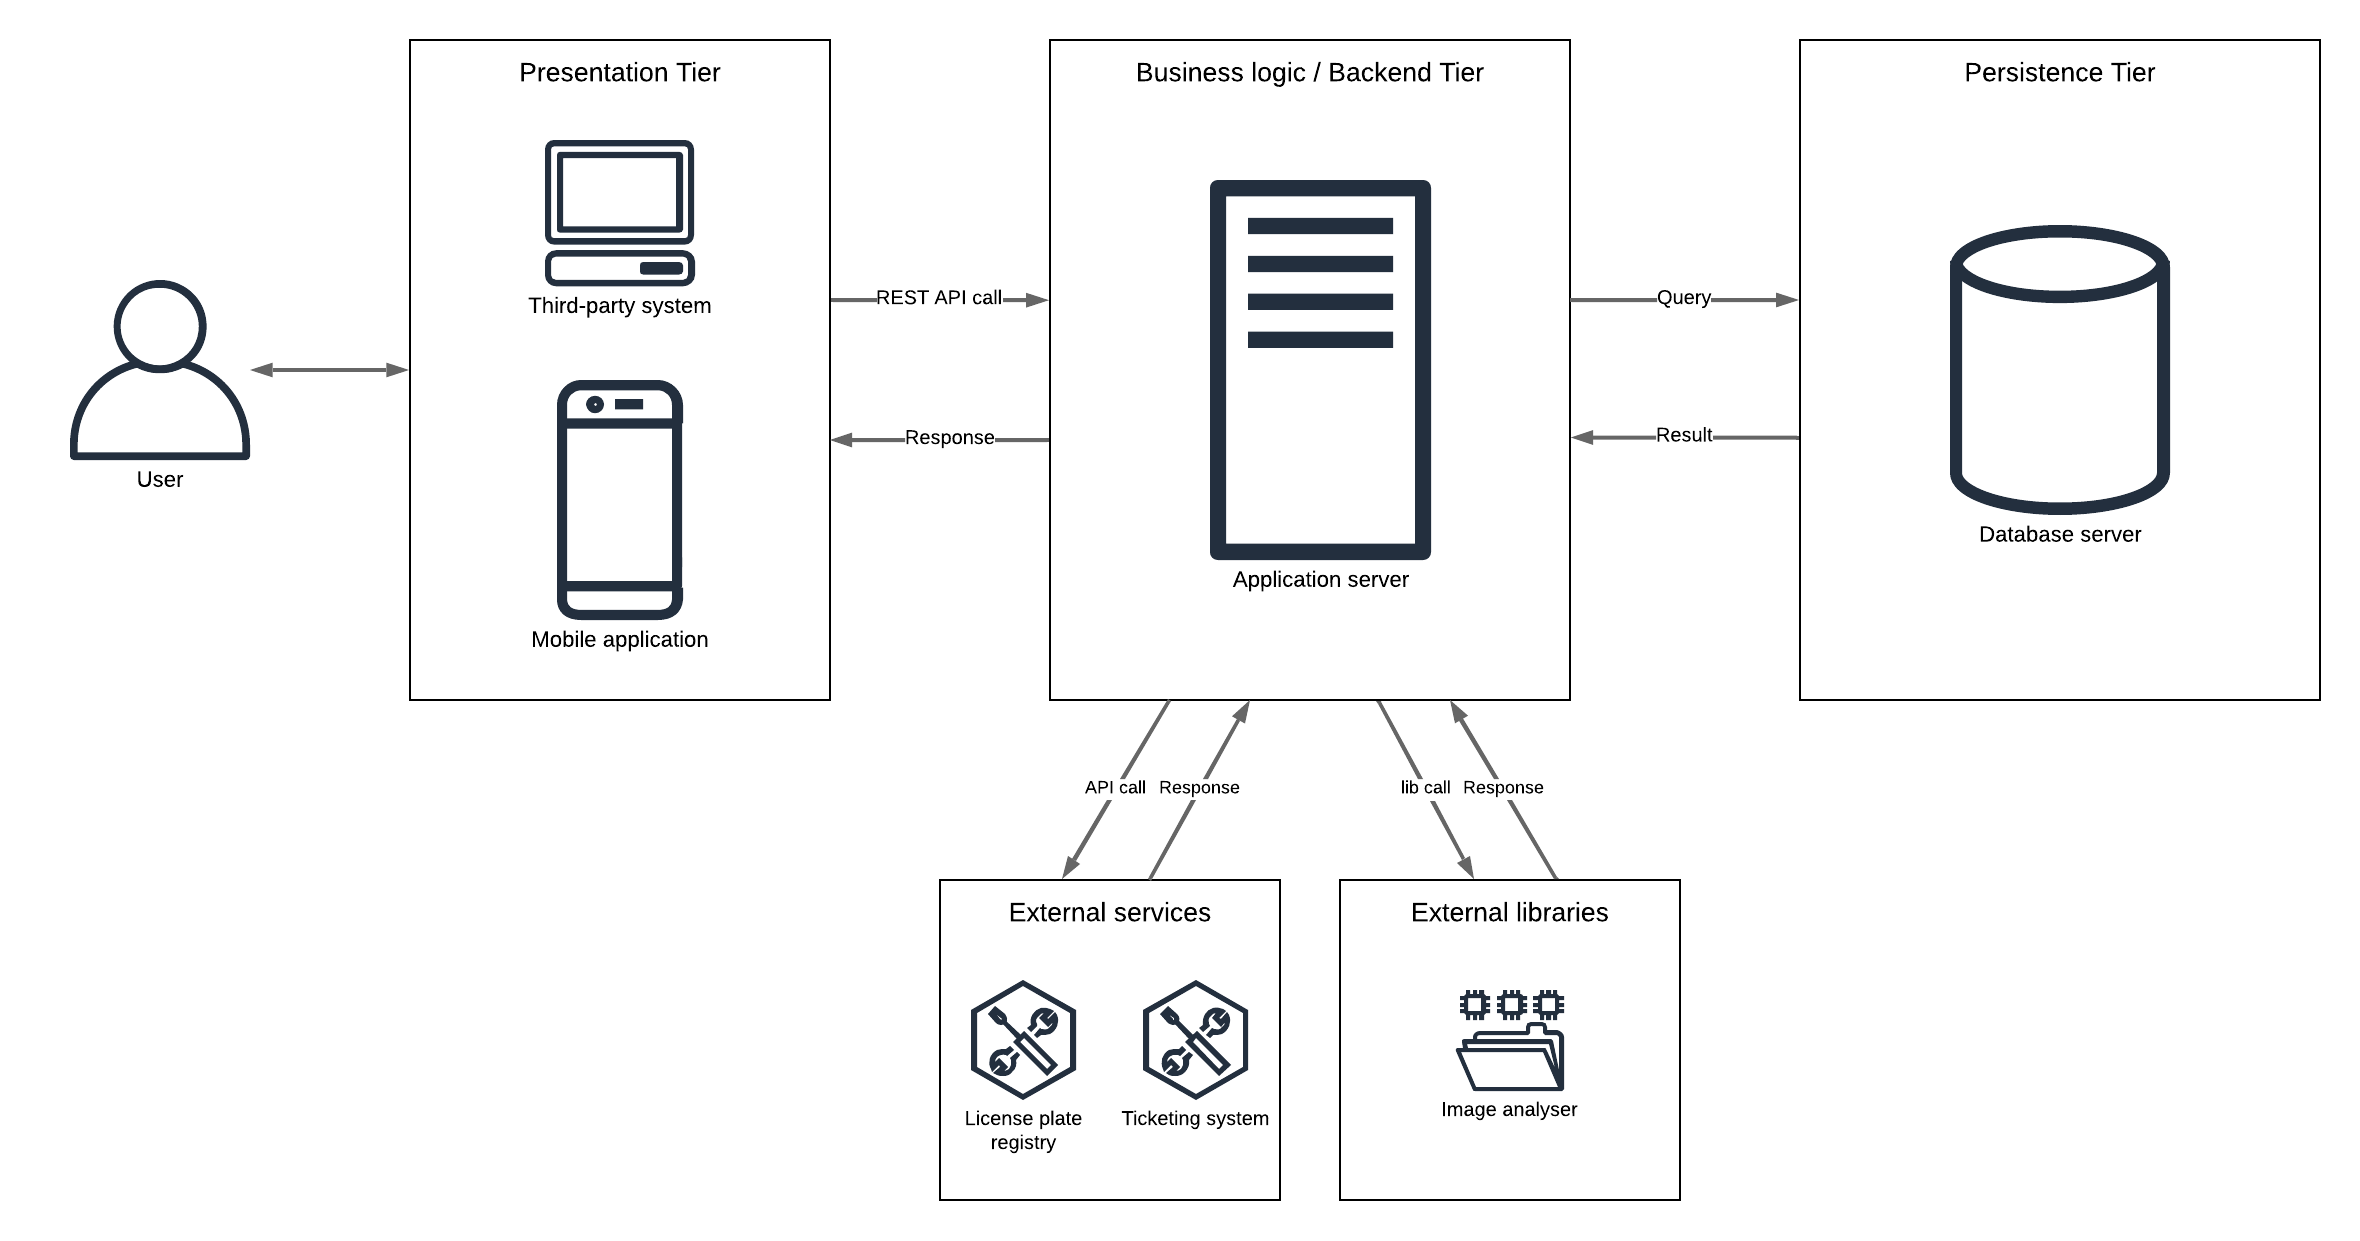
\includegraphics[width=0.8\textwidth]{Images/3tiers.png}}
\caption{\label{fig:3-tiers}Three tier architecture diagram.}
\end{figure}

The presentation tier is the only part of the system the user interacts with. Here is where the SafeStreets mobile application is located. The app provides a GUI for every user to interact with.
An alternative is for users to interact with the SafeStreets system through a third-party system, not developed by the team, which is capable of communicating with the application server via REST api calls.
Next is the business logic tier, where the core functionality of the system is provided. The backend presents a RESTful API, through which the presentation tier can communicate by making requests. This tier depends on external services that help in providing different functionalities, like the image analysis.
Last but not least, the persistence tier focuses on saving and managing the information gathered by the business logic. For this, a database management system is utilized. The only tier capable of accessing the persistence tier is the business logic, providing higher security for any sensitive data.


\subsection{Component view} \label{sub-sect:component-view}
The following diagrams describe the internal structure of the application server, which contains the business logic of the system. Users will communicate with it via its exposed interfaces, either with the mobile application or any system capable of performing HTTP requests.
Figure~\ref{fig:component-overview} shows a complete overview of the components to get a general idea of the structure. Following it, Figures \ref{fig:component-services-zoom} and \ref{fig:component-internal-zoom} zoom into parts of the diagram to appreciate the finer details.

\begin{figure}[H]
\centering
\fbox{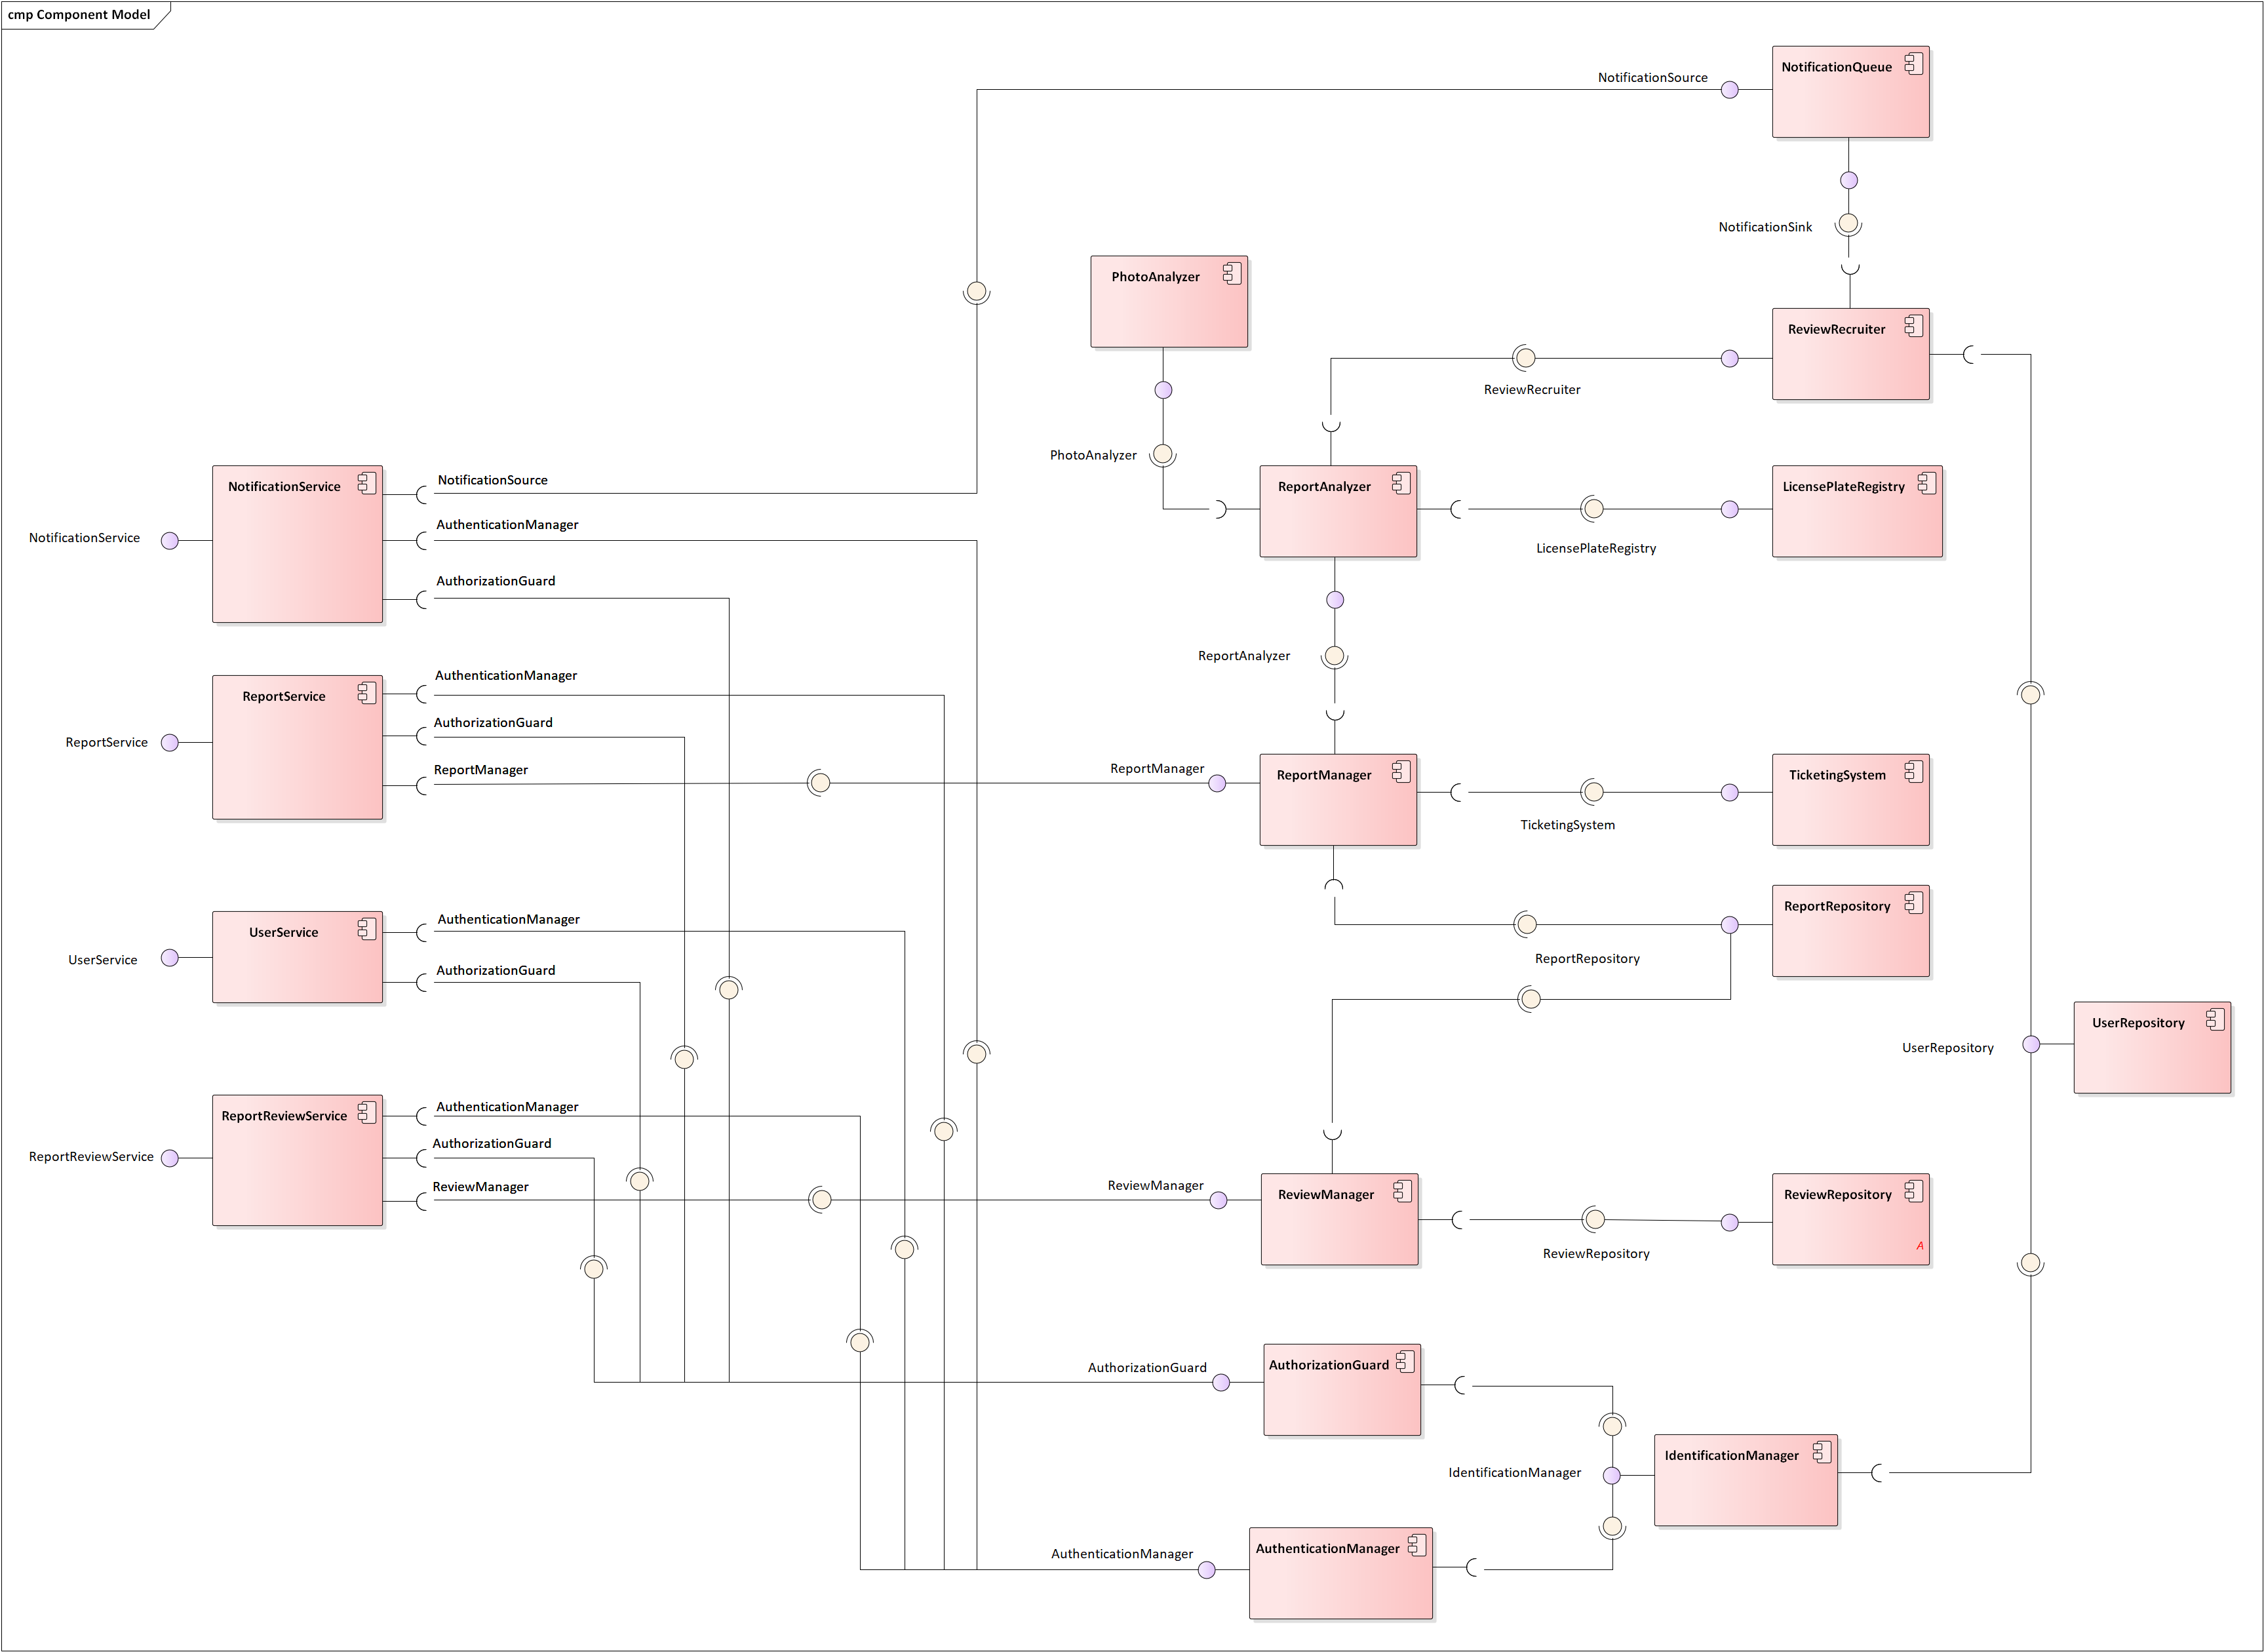
\includegraphics[angle=-90,origin=c, width=0.95\textwidth]{Images/architectural-design/Component Model.png}}
\caption{\label{fig:component-overview}Component model (Overview).}
\end{figure}

\begin{figure}[H]
    \centering
    \fbox{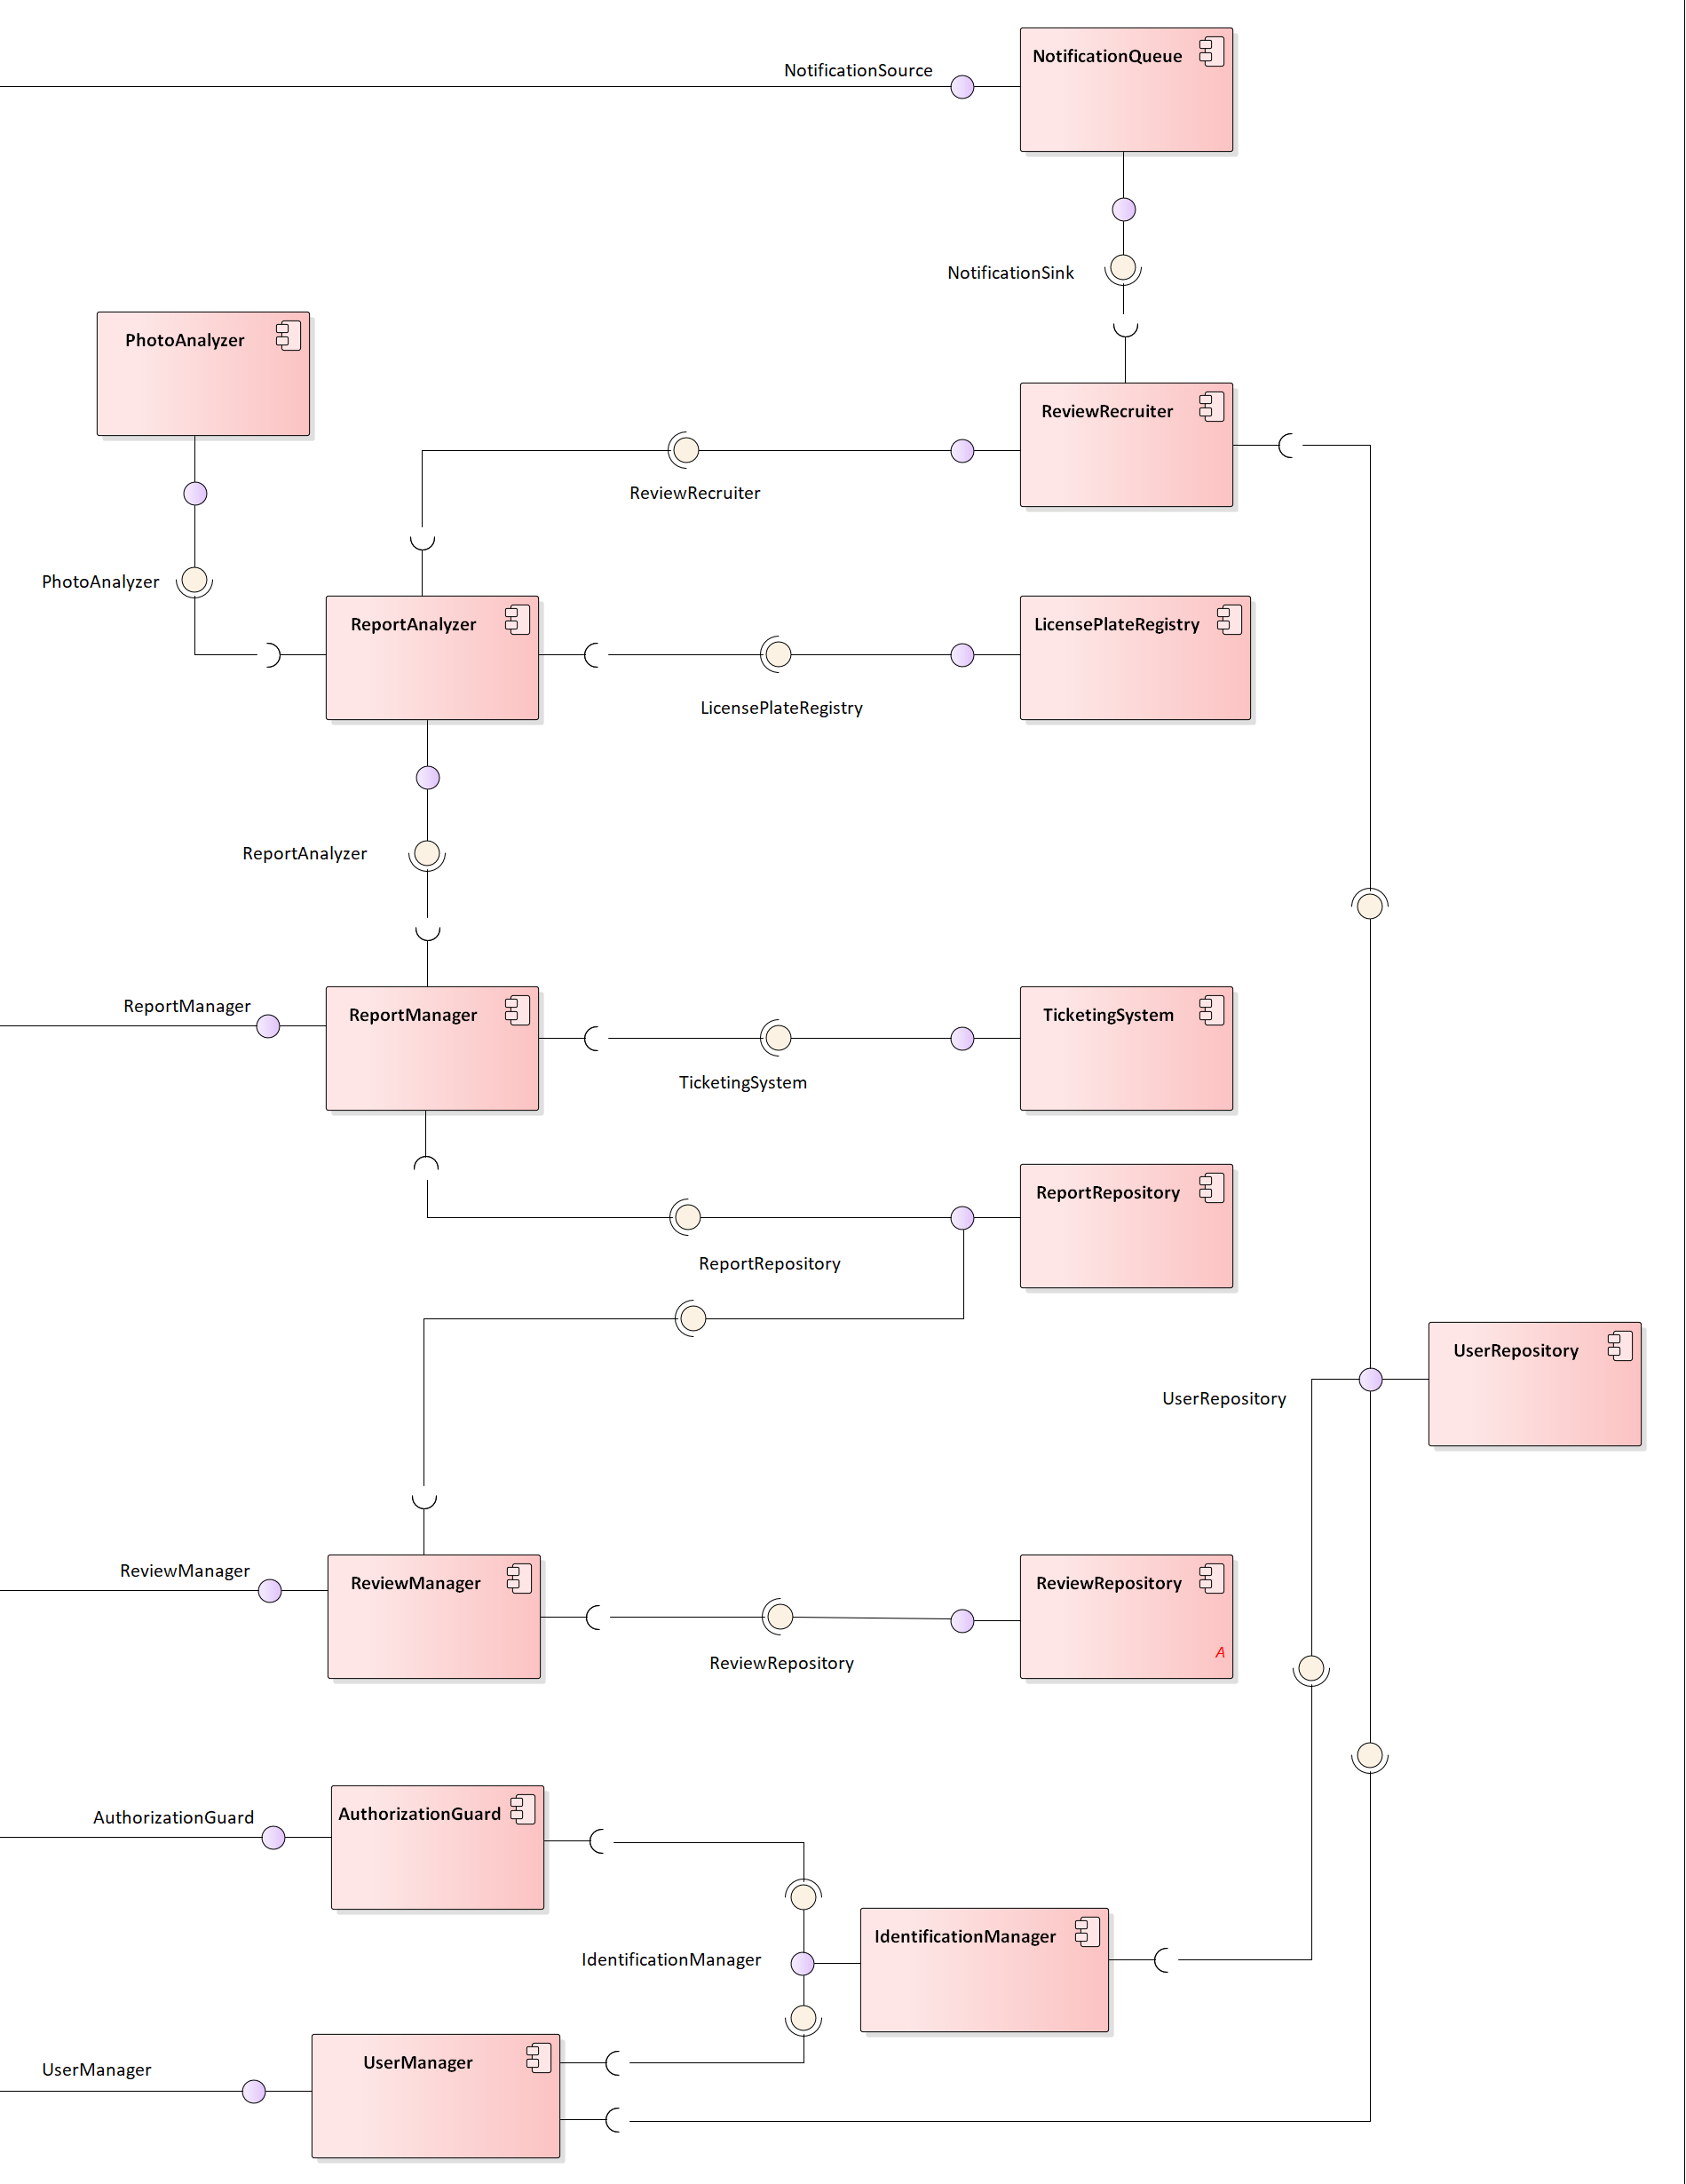
\includegraphics[width=0.95\textwidth]{Images/architectural-design/Component Model - Internal Zoom.png}}
    \caption{\label{fig:component-internal-zoom}Component model (Application server internals zoom-in).}
\end{figure}

Figure~\ref{fig:component-internal-zoom} shows the components responsible for the application business logic, mainly report submission and analysis, but also authorization and authentication.
The purpose of each component is the following (going top-down, left-right):
\begin{itemize}
    \item NotificationQueue: queues notifications to users so they can be received in the order they were generated when the user requests them.
    \item PhotoAnalyzer: detects license plate in a given photograph along with the car it is attached to.
    \item ReviewRecruiter: recruits users to review a given photograph with poor license plate detection by sending them notifications.
    \item ReportAnalyzer: takes a submitted report and performs an analysis on it to determine its validity and confidence in its veracity. 
    \item LicensePlateRegistry: communicates with the external license plate registry to obtain information about a car given a license plate.
    \item ReportManager: contains the logic needed to satisfy report submissions and queries.
    \item TicketingSystem: communicates with the external ticketing system to obtain ticket information about a given license plate.
    \item ReportRepository: handles interaction with the DBMS regarding reports.
    \item UserRepository: handles interaction with the DBMS regarding users.
    \item ReviewManager: manages review submissions and updates the status of a reviewed report accordingly.
    \item ReviewRepository: handles interaction with the DBMS regarding reviews
    \item AuthorizationGuard: checks whether a given token or API key is authorized to perform a certain request.
    \item IdentificationManager: assigns identification tokens and can extract information from them, used for authentication purposes.
    \item UserManager: responsible for the authentication flow needed to use the application, registering as a new user, logging in, obtaining profile information and editing such information.
\end{itemize}

\begin{figure}[H]
    \centering
    \fbox{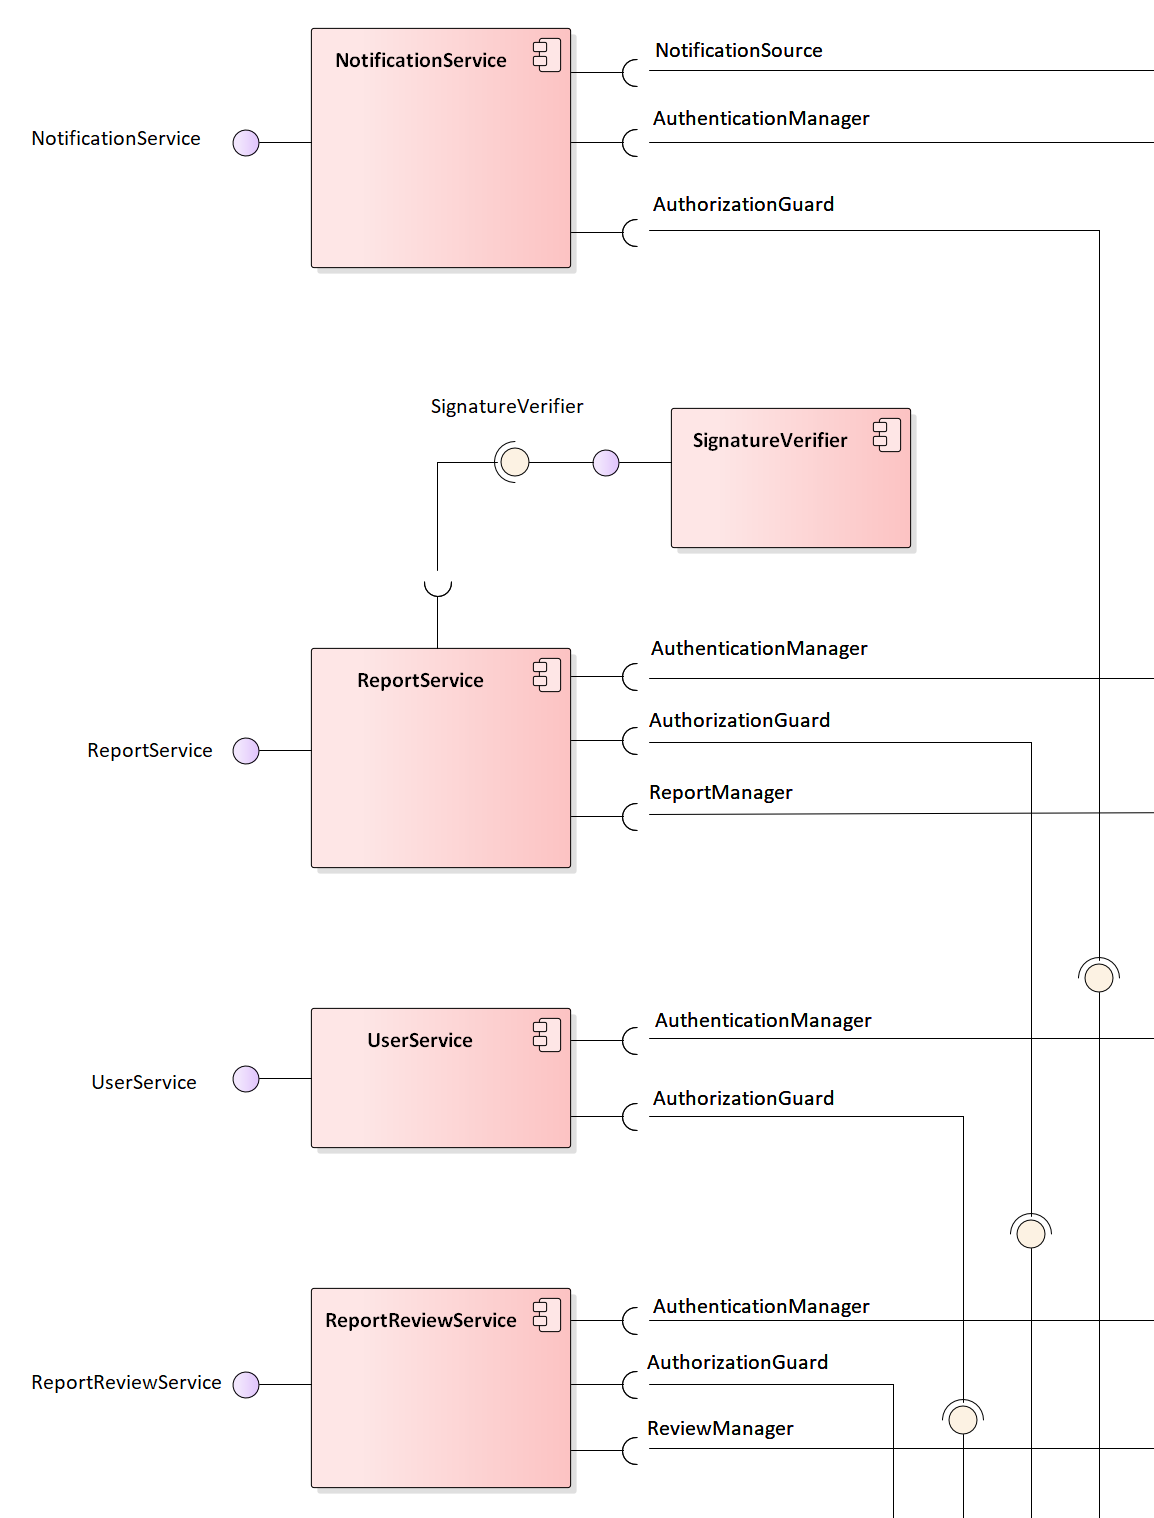
\includegraphics[width=0.95\textwidth]{Images/architectural-design/Component Model - Services Zoom.png}}
    \caption{\label{fig:component-services-zoom}Component model (Services zoom-in).}
\end{figure}

Figure~\ref{fig:component-services-zoom} goes into the four services exposed by the application server. These provide the functionality needed to the mobile application and allow other systems to integrate to SafeStreets.
To identify who is performing the request and maintain security, all services are connected to and use the AuthorizationGuard and UserManager.
The services (from top to bottom) provide the following functionality:
\begin{itemize}
    \item NotificationService: allows a user to obtain their pending notifications.
    \item ReportService: report submissions and queries of report data.
    \item UserService: authentication flow to identify a user of the mobile application.
    \item ReportReviewService: submissions of report reviews.
\end{itemize}


\subsection{Deployment view}

As stated previously, the system presents a three tier architecture.
\begin{itemize}
    \item Tier 1 is the presentation tier, where the mobile app is installed on compatible Android or iOS phones. Distribution of the appropriate executable would be handled by the corresponding app stores. Deployment on both platforms is important to be able to reach the greatest amount of possible users.
    \item Tier 2 contains the business logic and is the home of the application server. To facilitate deployment and testing under controlled conditions, the executable itself is isolated from the underlying server OS through Docker. This minimizes the setup needed after a container is built and avoids any possible conflict with the OS.
    \item Tier 3, persistence, includes the database management system, which is again deployed using a docker container because of all the advantages stated before. 
\end{itemize}

\begin{figure}[H]
    \centering
    \fbox{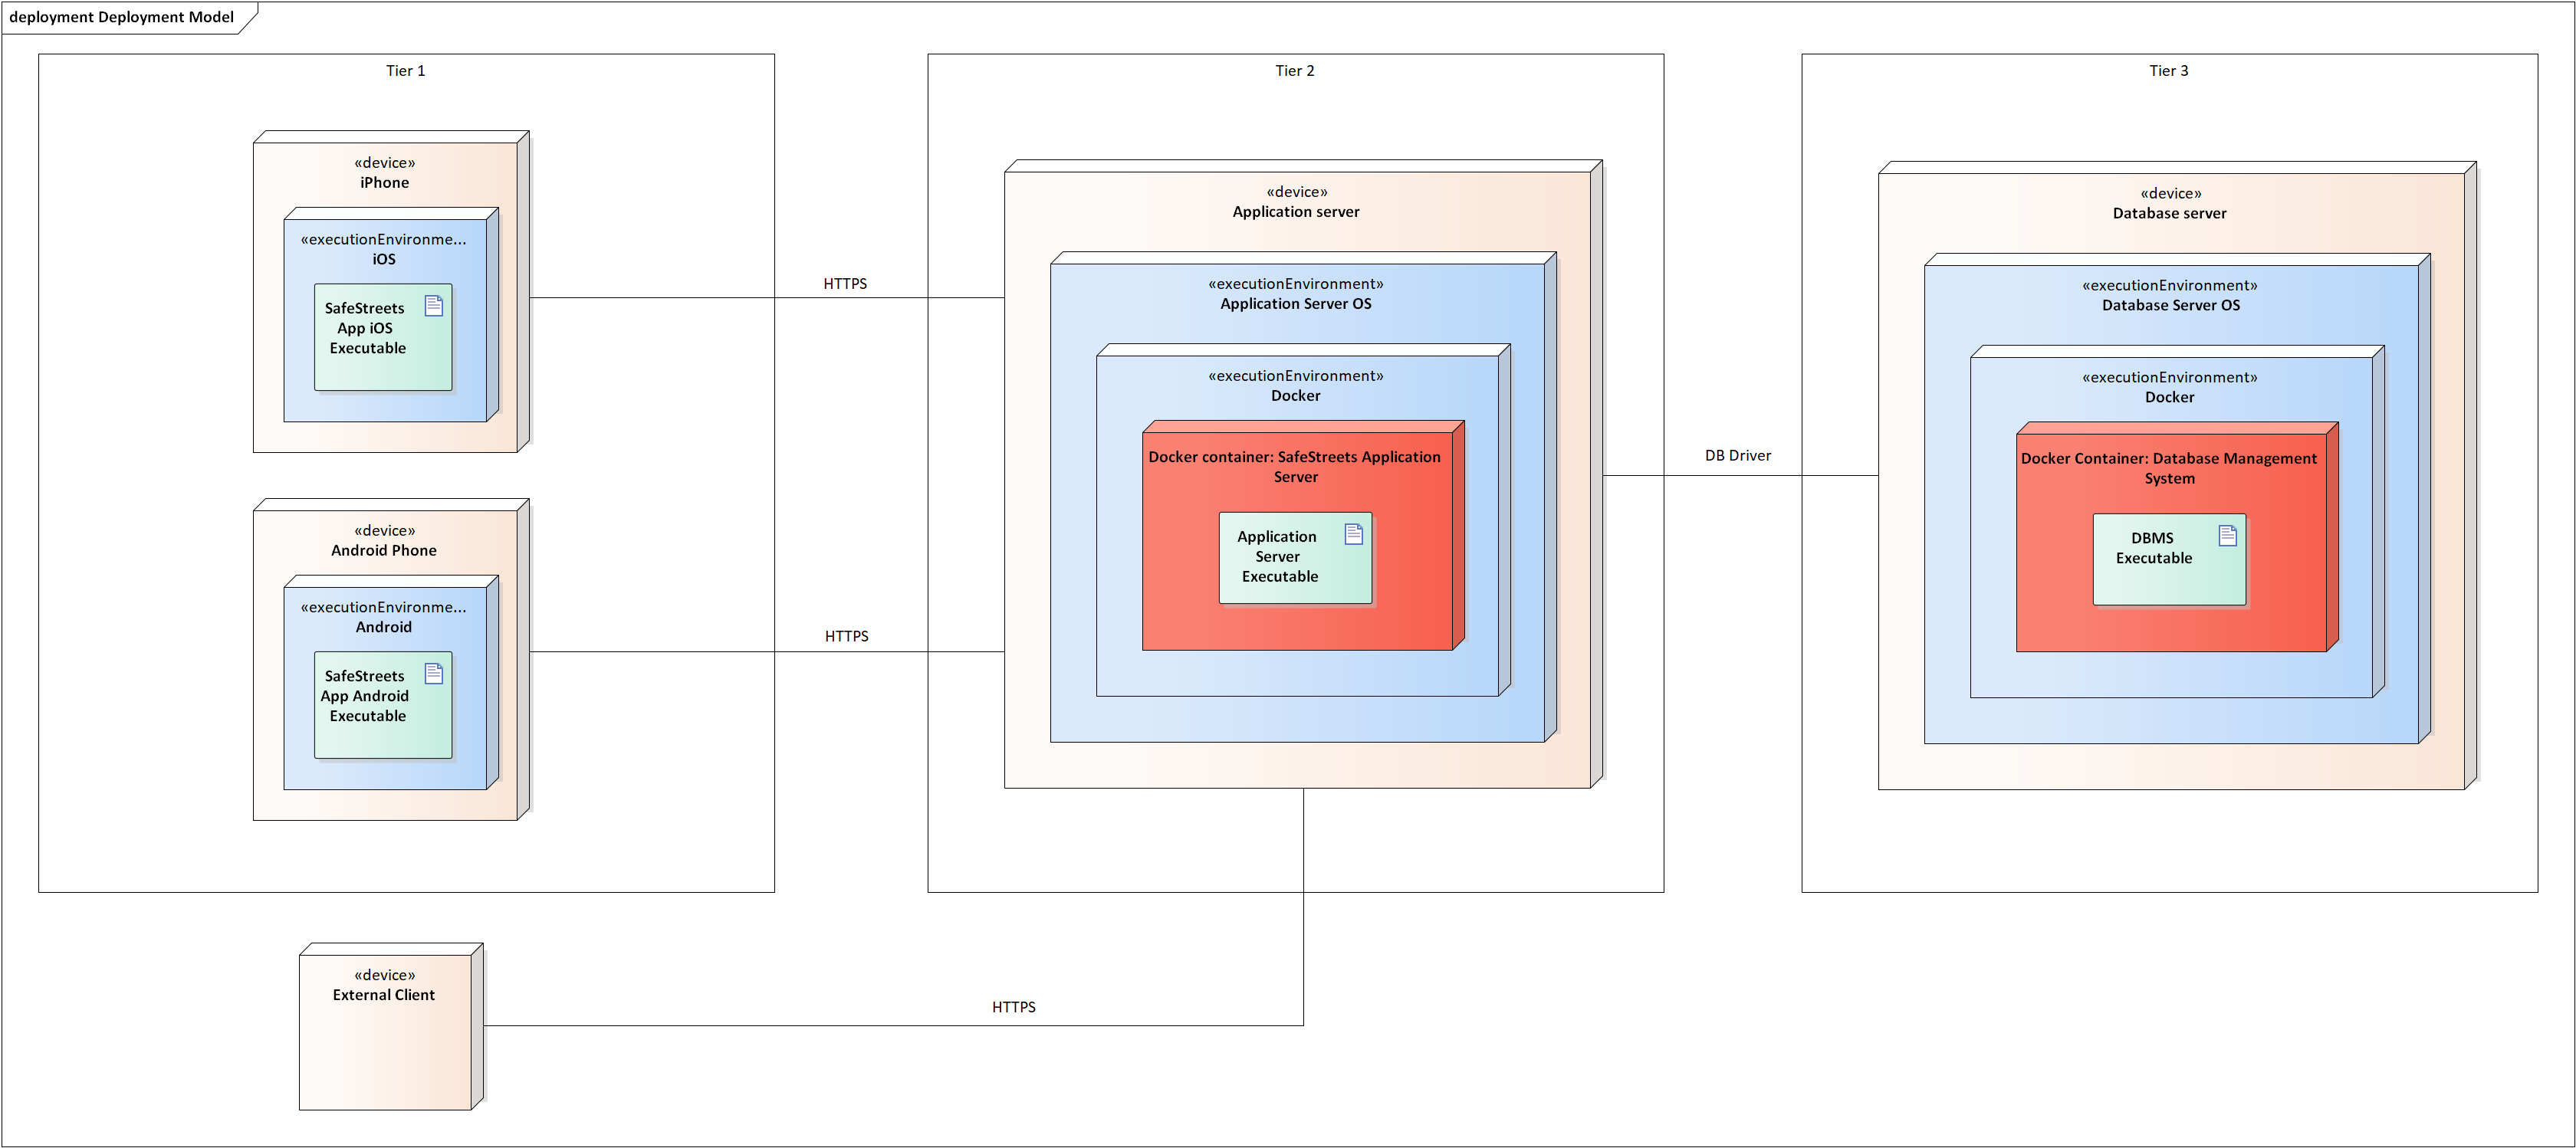
\includegraphics[angle=-90,origin=c, height=0.7\textheight]{Images/architectural-design/Deployment Model.png}}
    \caption{\label{fig:deployment-diagram}Deployment diagram.}
\end{figure}

Figure~\ref{fig:deployment-diagram} shows a diagram of the deployment of all three tiers, along with their form of communication, which consists of HTTPS from the mobile application to the business logic tier, and the corresponding database driver from the business logic tier to the persistence tier. 

External to the system a separate device is depicted, indicating third party system or some other kind of API user, communicating directly with the application server via HTTPS.

\subsection{Runtime view}
To avoid repetition and explain each process more clearly, the first two sequence diagrams present the authorization procedures that are executed by all services on each request. These are needed to guarantee that whoever is performing a request has the proper authorization and the system can answer it. 
As this process is not tied to a particular component, a generic “Service” component represents the corresponding service answering the request and a “SystemComponent” is what the service will be using to generate the response.

\subsubsection{Token authorization}
In this sequence, the general process of authorizing a user request through a token is shown. This process is executed by each and every one of the services that provide a token interface to the user. Any particular action has an access level that needs to be equal or lesser than the token access level, this is checked by the AuthorizationGuard, which asks the IdentificationManager for information about the token.
If this is correct and the user is found, then the action is executed by the corresponding system component.
\begin{figure}[H]
    \centering
    \fbox{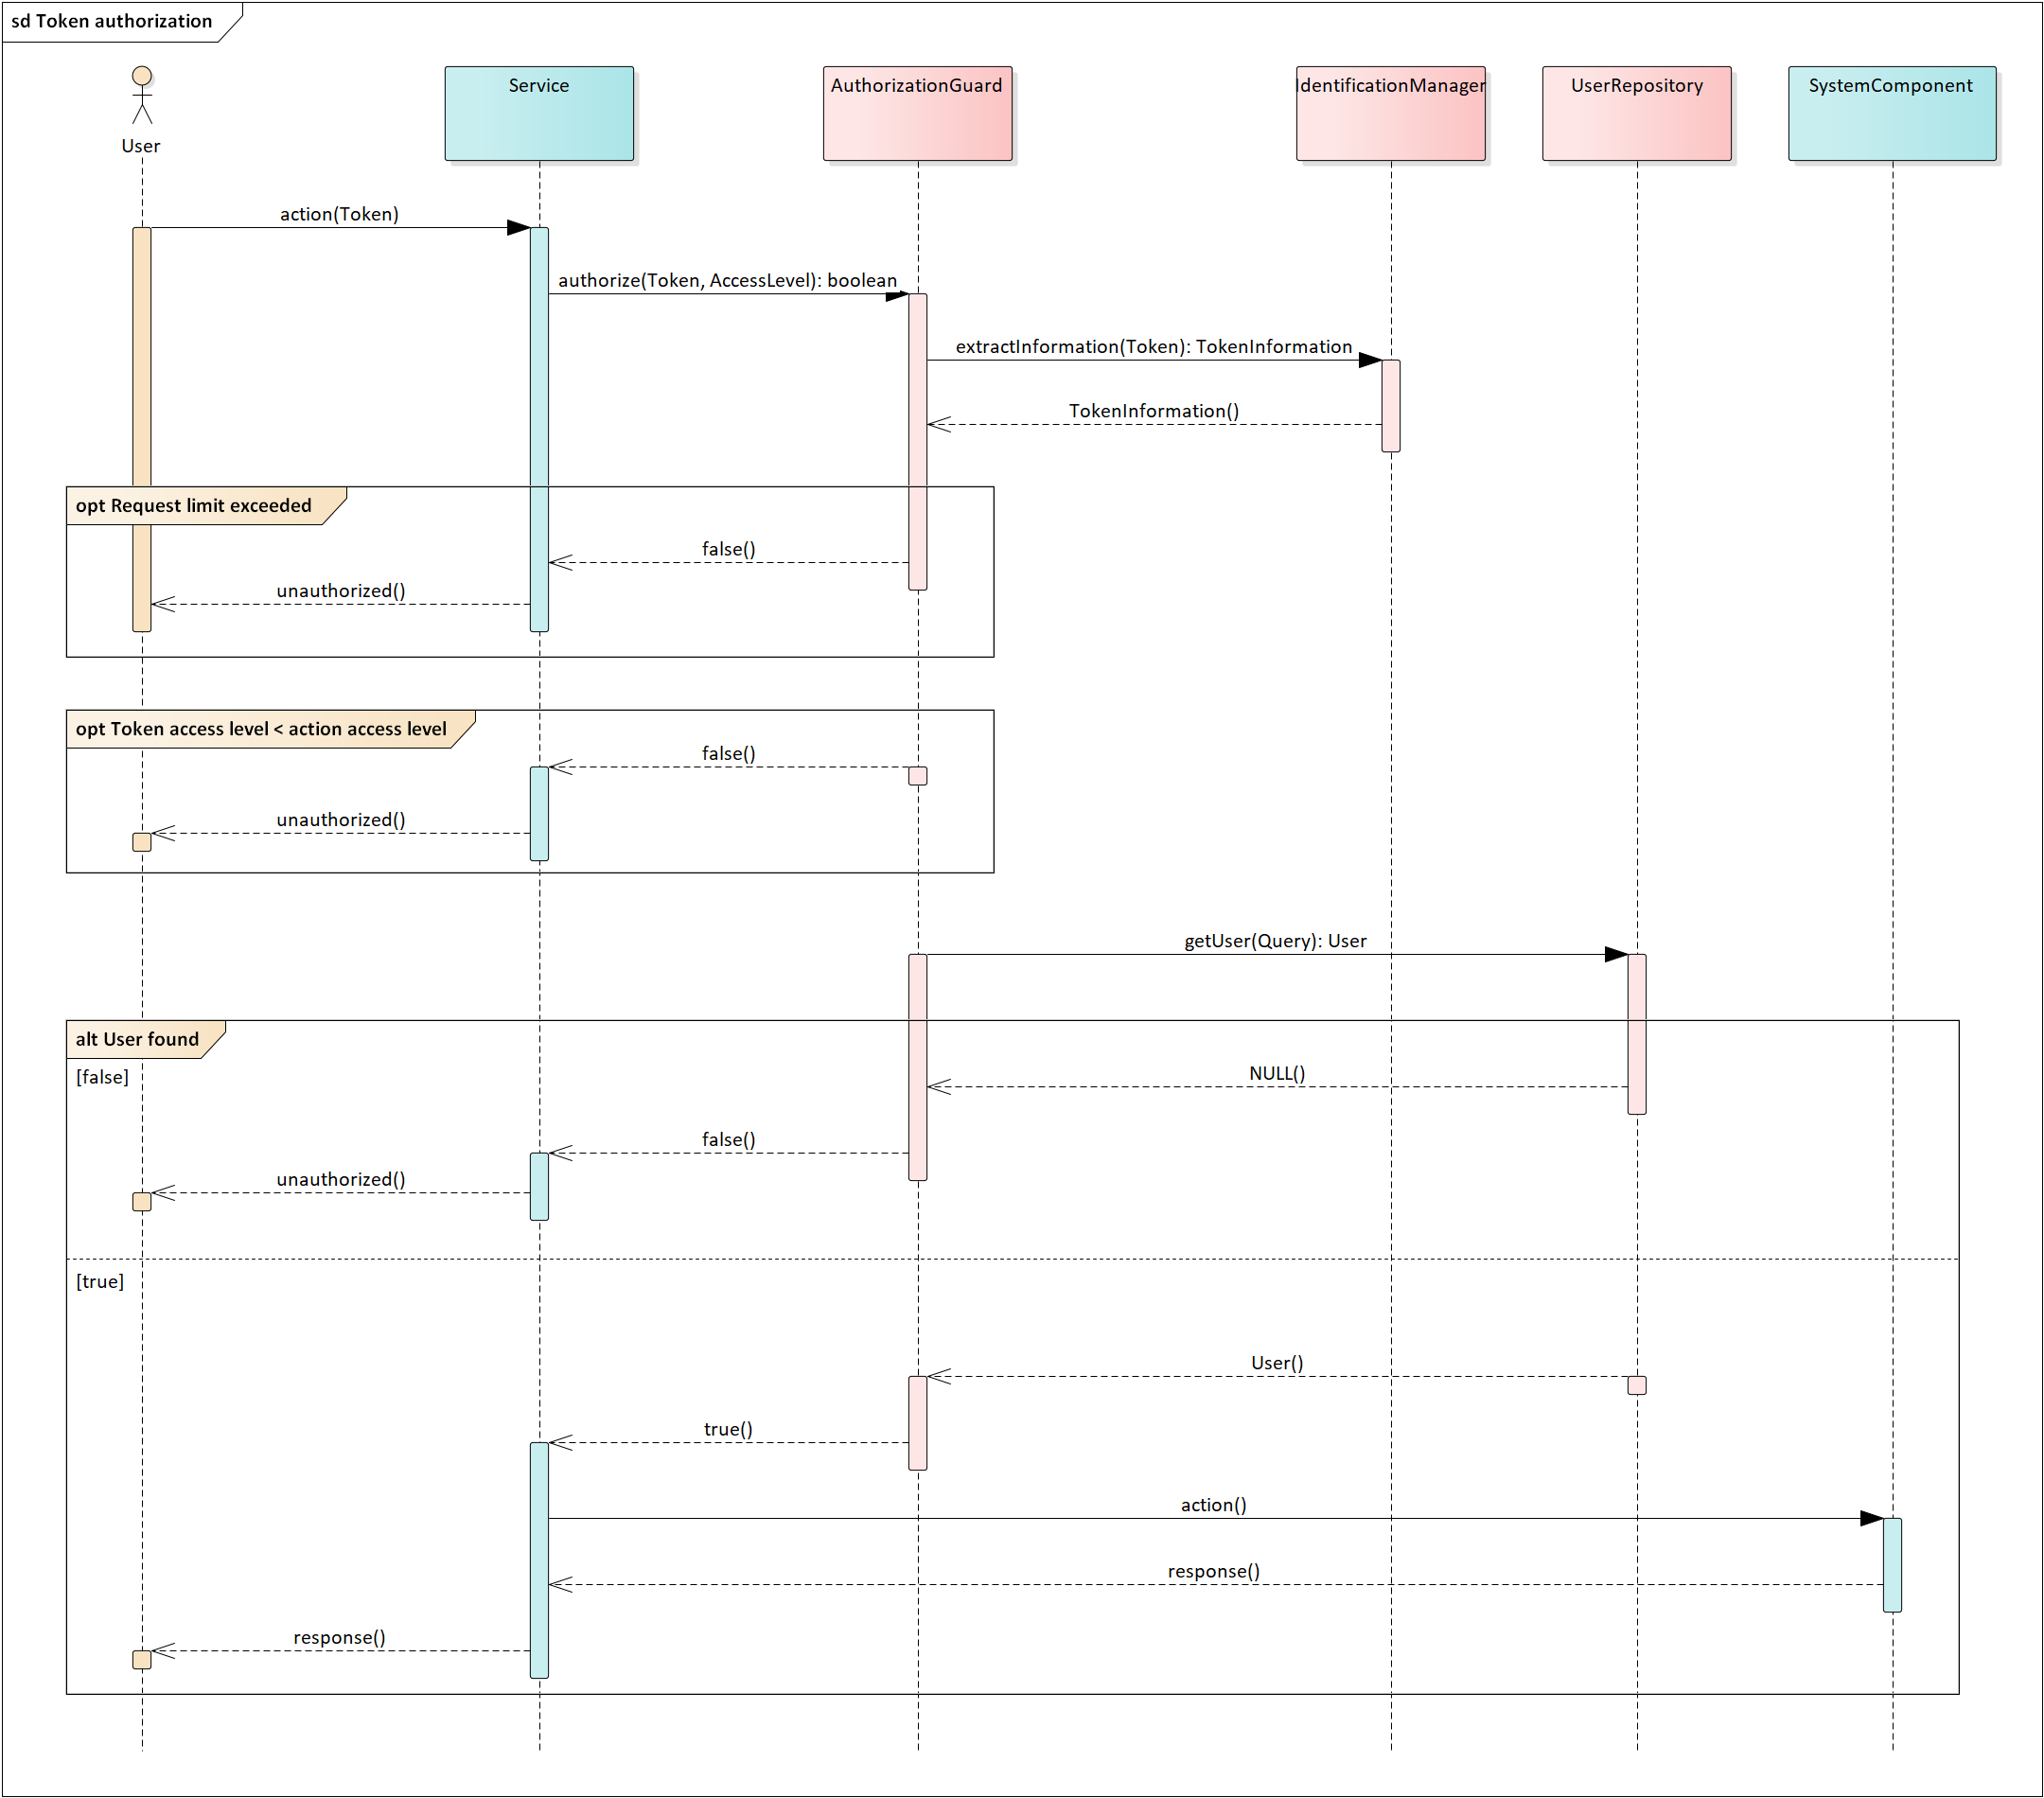
\includegraphics[angle=-90, origin=c, width=0.98\textwidth]{Images/architectural-design/Sequence/1-Token authorization.png}}
    \caption{\label{fig:sequence-token-auth}Sequence diagram - Token authorization.}
\end{figure}

\subsubsection{Key authorization}
If the user wants to make use of the public API, then instead of a token, an API key is provided. As with the token authorization, this is performed by every service that provides an interface with an API key. The process is the same as before with the difference that since the user is not logged into the application, it does not have to be retrieved from the system. Also, the possible actions performed through the public API do not need to identify the user performing them as they consist of queries only.
\begin{figure}[H]
    \centering
    \fbox{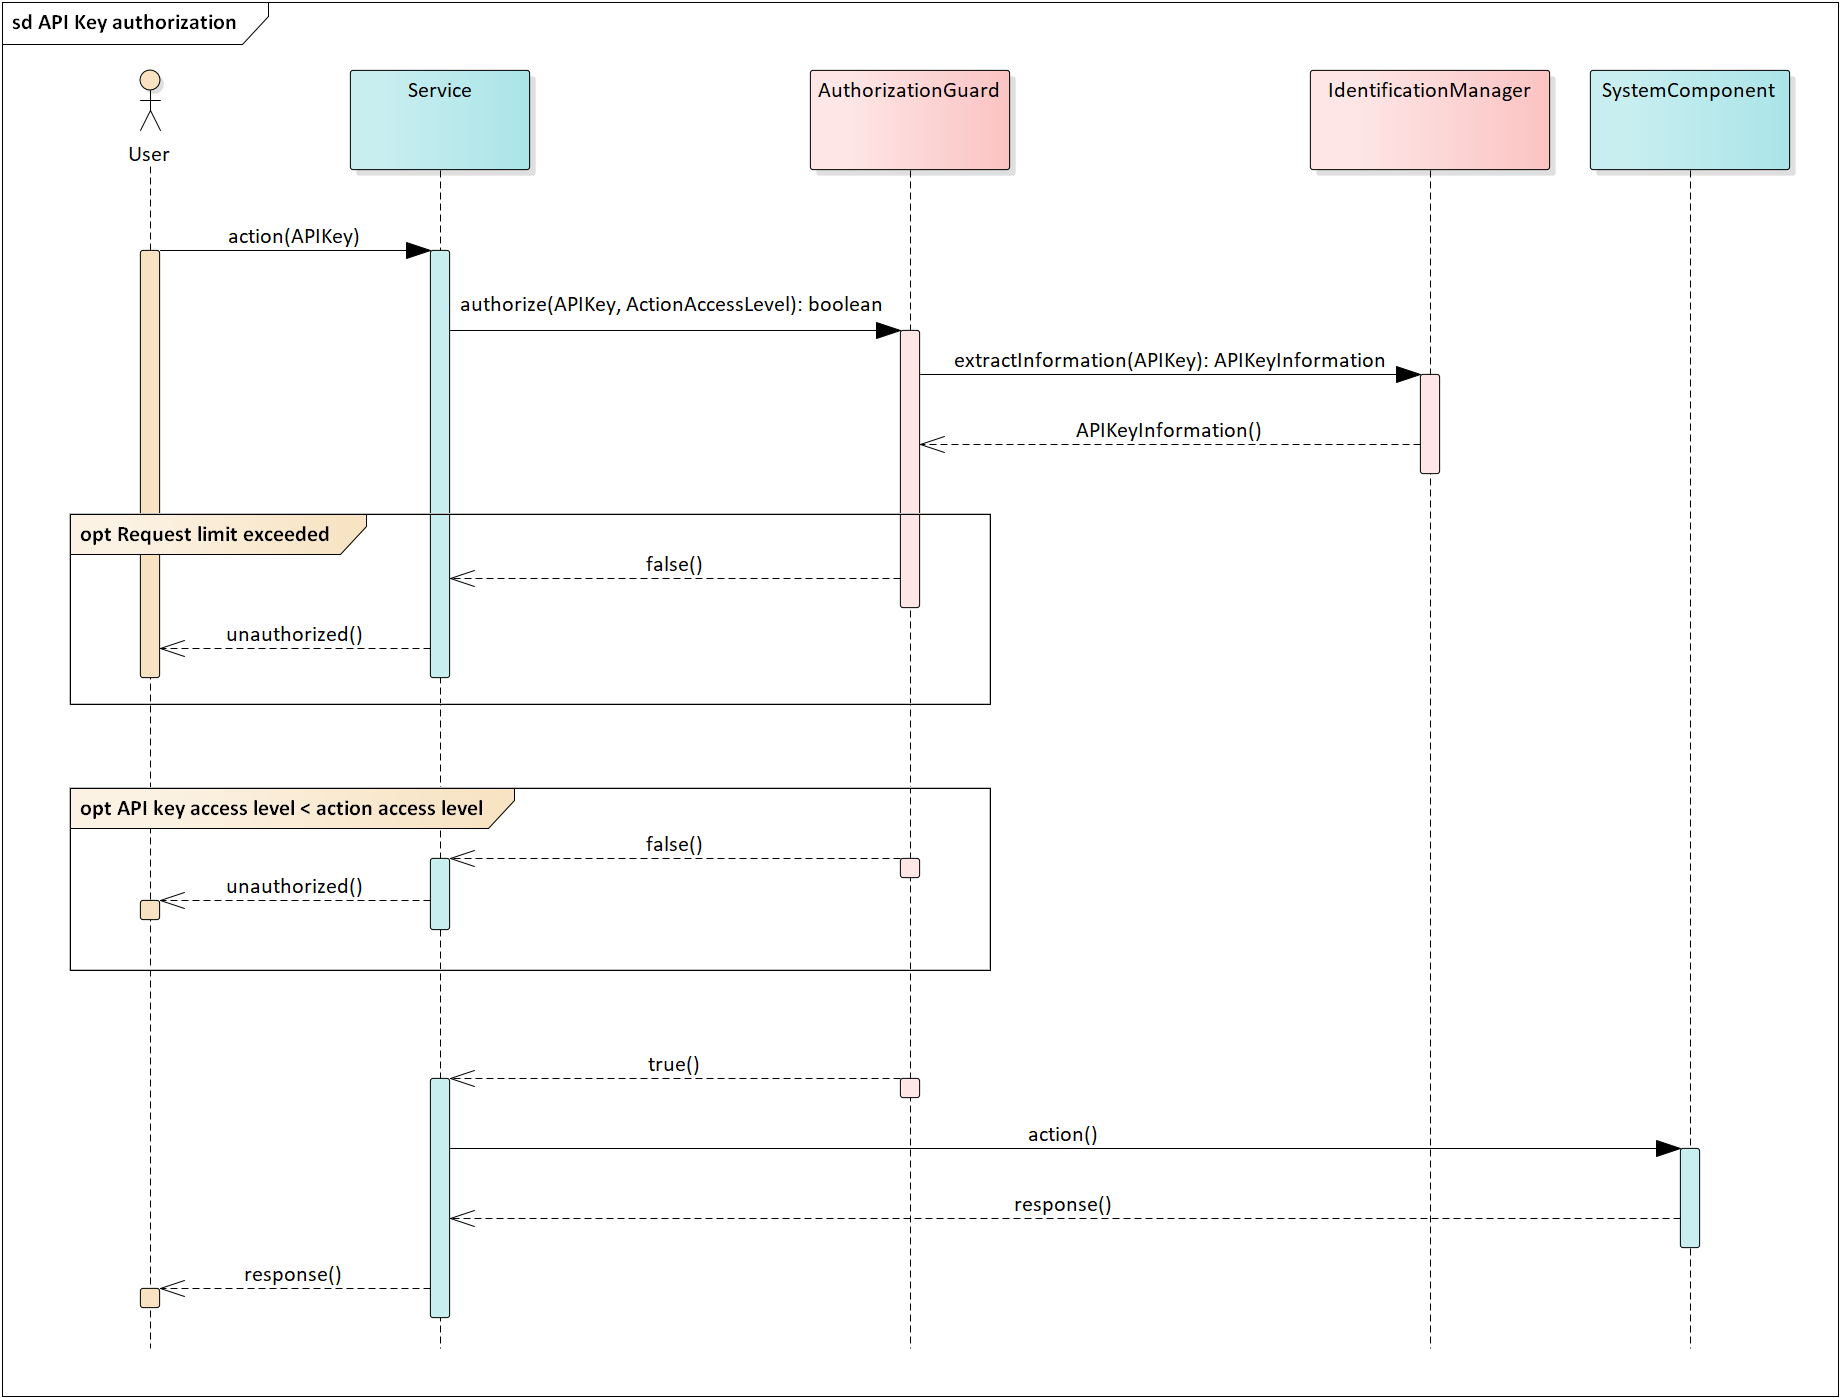
\includegraphics[angle=-90, origin=c, width=0.98\textwidth]{Images/architectural-design/Sequence/2-API Key authorization.png}}
    \caption{\label{fig:sequence-api-key-auth}Sequence diagram - API Key authorization.}
\end{figure}

\subsubsection{Report submission}
The following sequence describes the process of submitting a report.
The ReportService is in charge of executing the action. First of all, it gets the user from the UserManager through the token and gives the order to the ReportManager to submit the report. The ReportManager gets the ReportAnalyzer to analyse the report. If the report is invalid, then it is saved through the ReportRepository with an explanation of the error and an error message is returned to the user. If the report is valid, then it is saved along with the analysis result and an ok code is returned to the user.

\begin{figure}[H]
    \centering
    \fbox{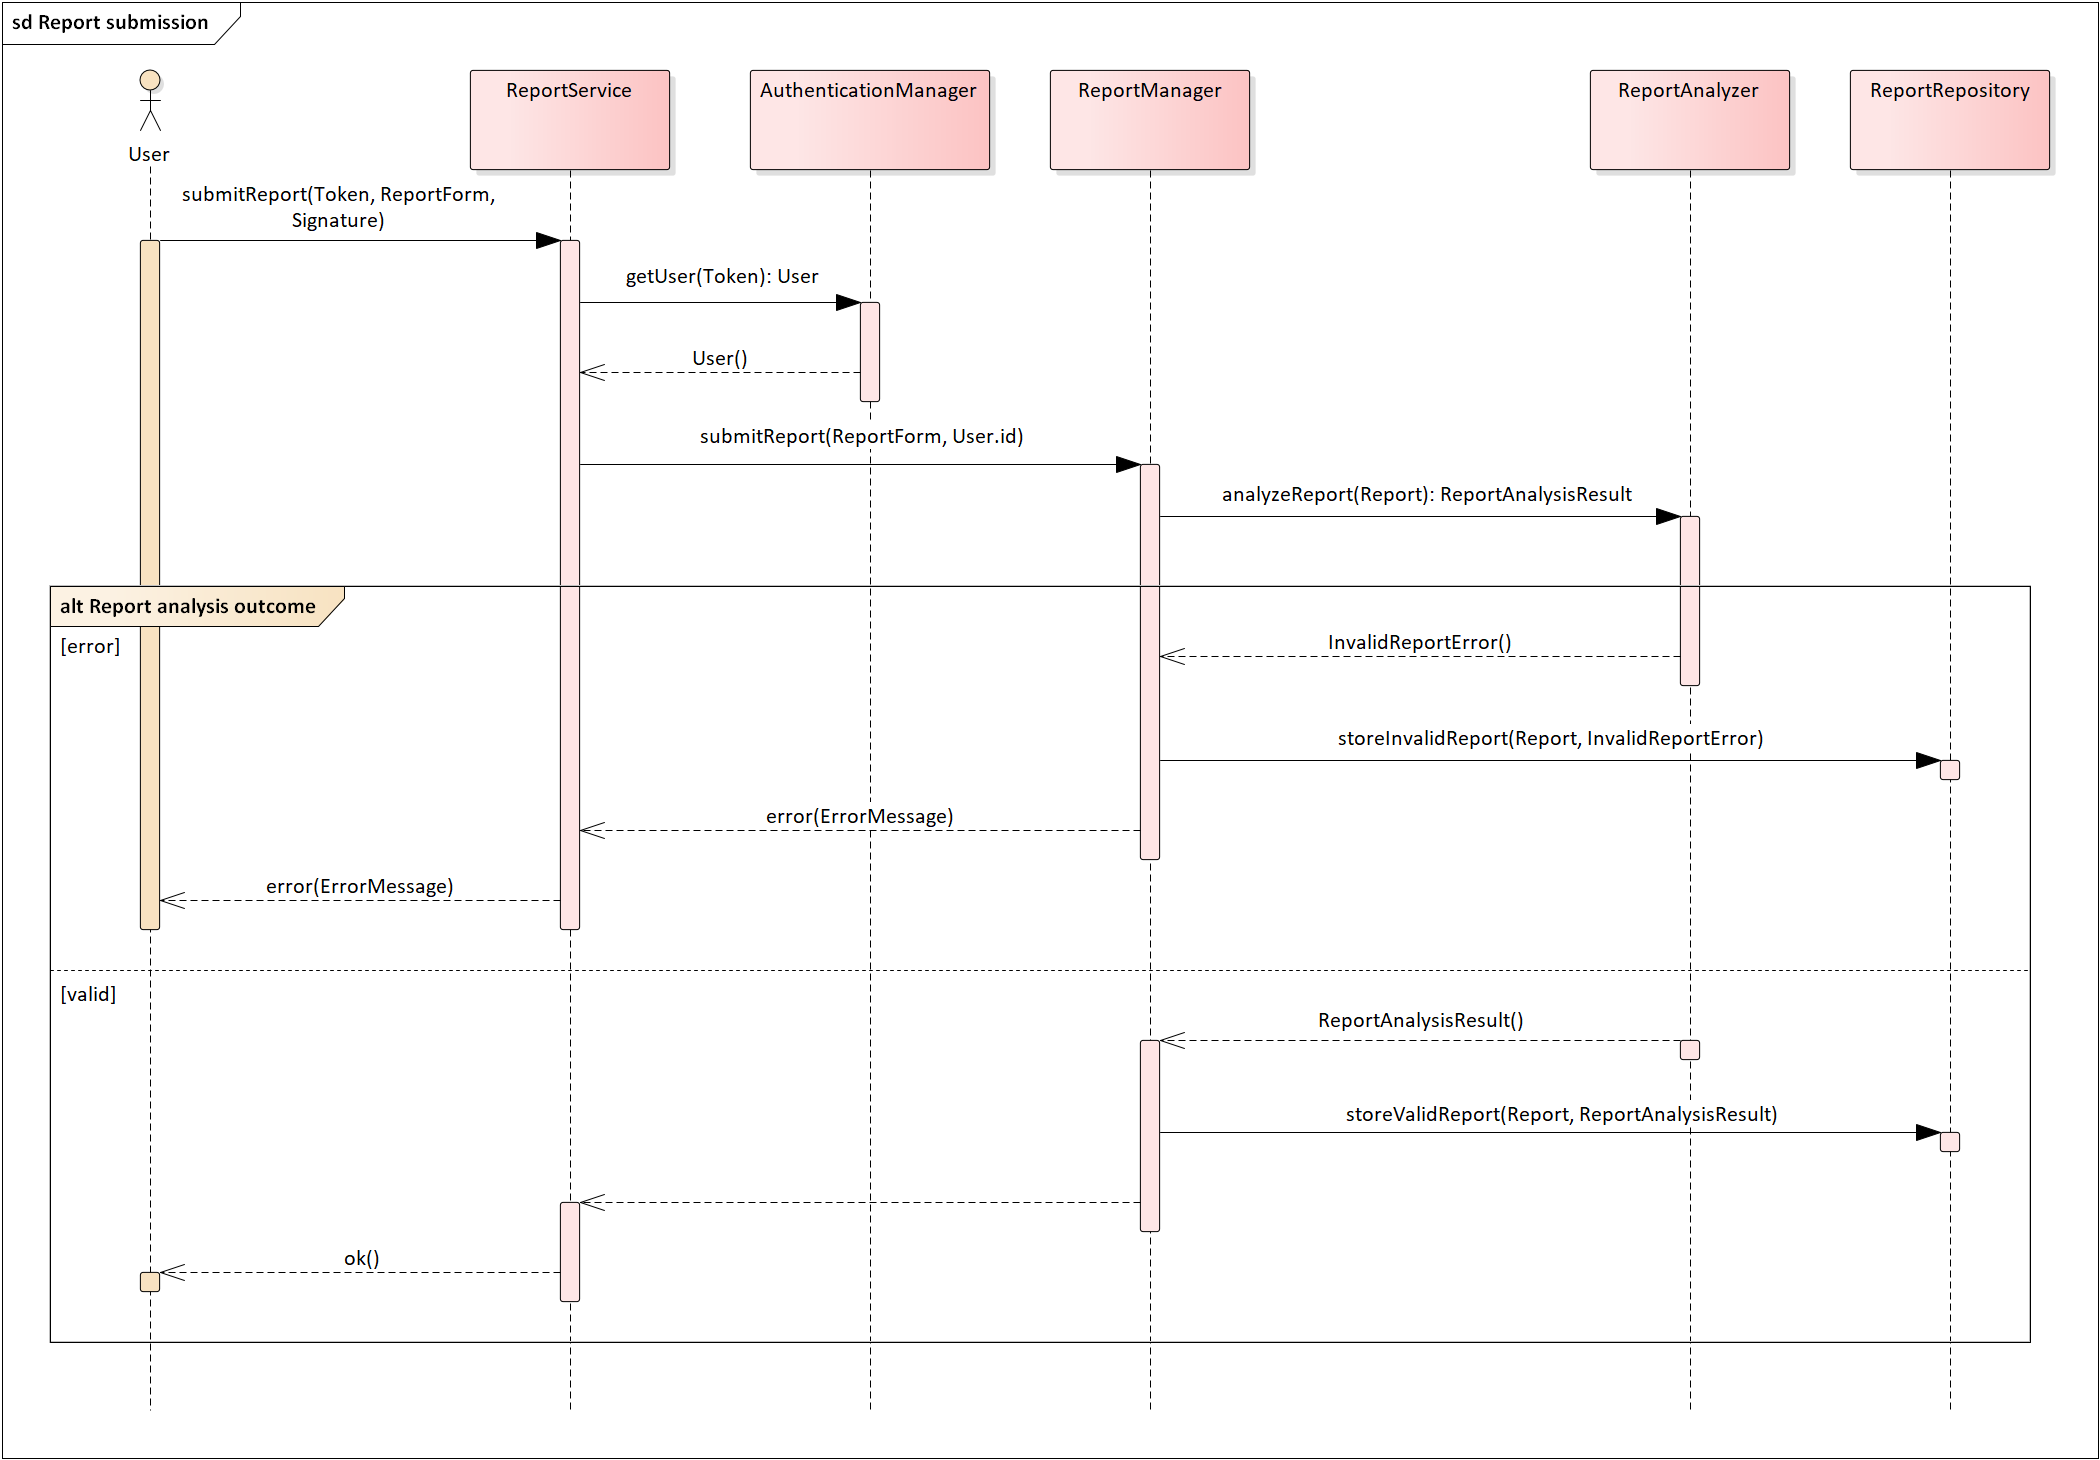
\includegraphics[angle=-90, origin=c, width=0.8\textwidth]{Images/architectural-design/Sequence/3-Report submission.png}}
    \caption{\label{fig:sequence-report-submission}Sequence diagram - Report submission.}
\end{figure}

\subsubsection{Report analysis}
Here the previously mentioned report analysis is explained with more detail.
The ReportManager gives a report to the ReportAnalyser for its analysis.
The ReportAnalyser uses the PhotoAnalyser to get car and license plate detections from the report photo. The report is considered invalid and an error is returned if no license plates are detected, if none of them match with the one provided in the report or if no cars are detected. If a licence plate matches but the confidence of the PhotoAnalyser analysis is below 80\%, then the report is sent to the ReviewRecruiter for user review and an in-review result is returned to the ReportManager.
The car detection is also required to have a confidence of at least 80\%, or the analysis result is low-confidence. If the car detection is ok, then the LicensePlateRegistry is consulted for information about the car with the detected license plate. This information is compared with the detected car; if they match, the result is a high-confidence report, if they do not, the result is a low-confidence report.

\begin{figure}[H]
    \centering
    \fbox{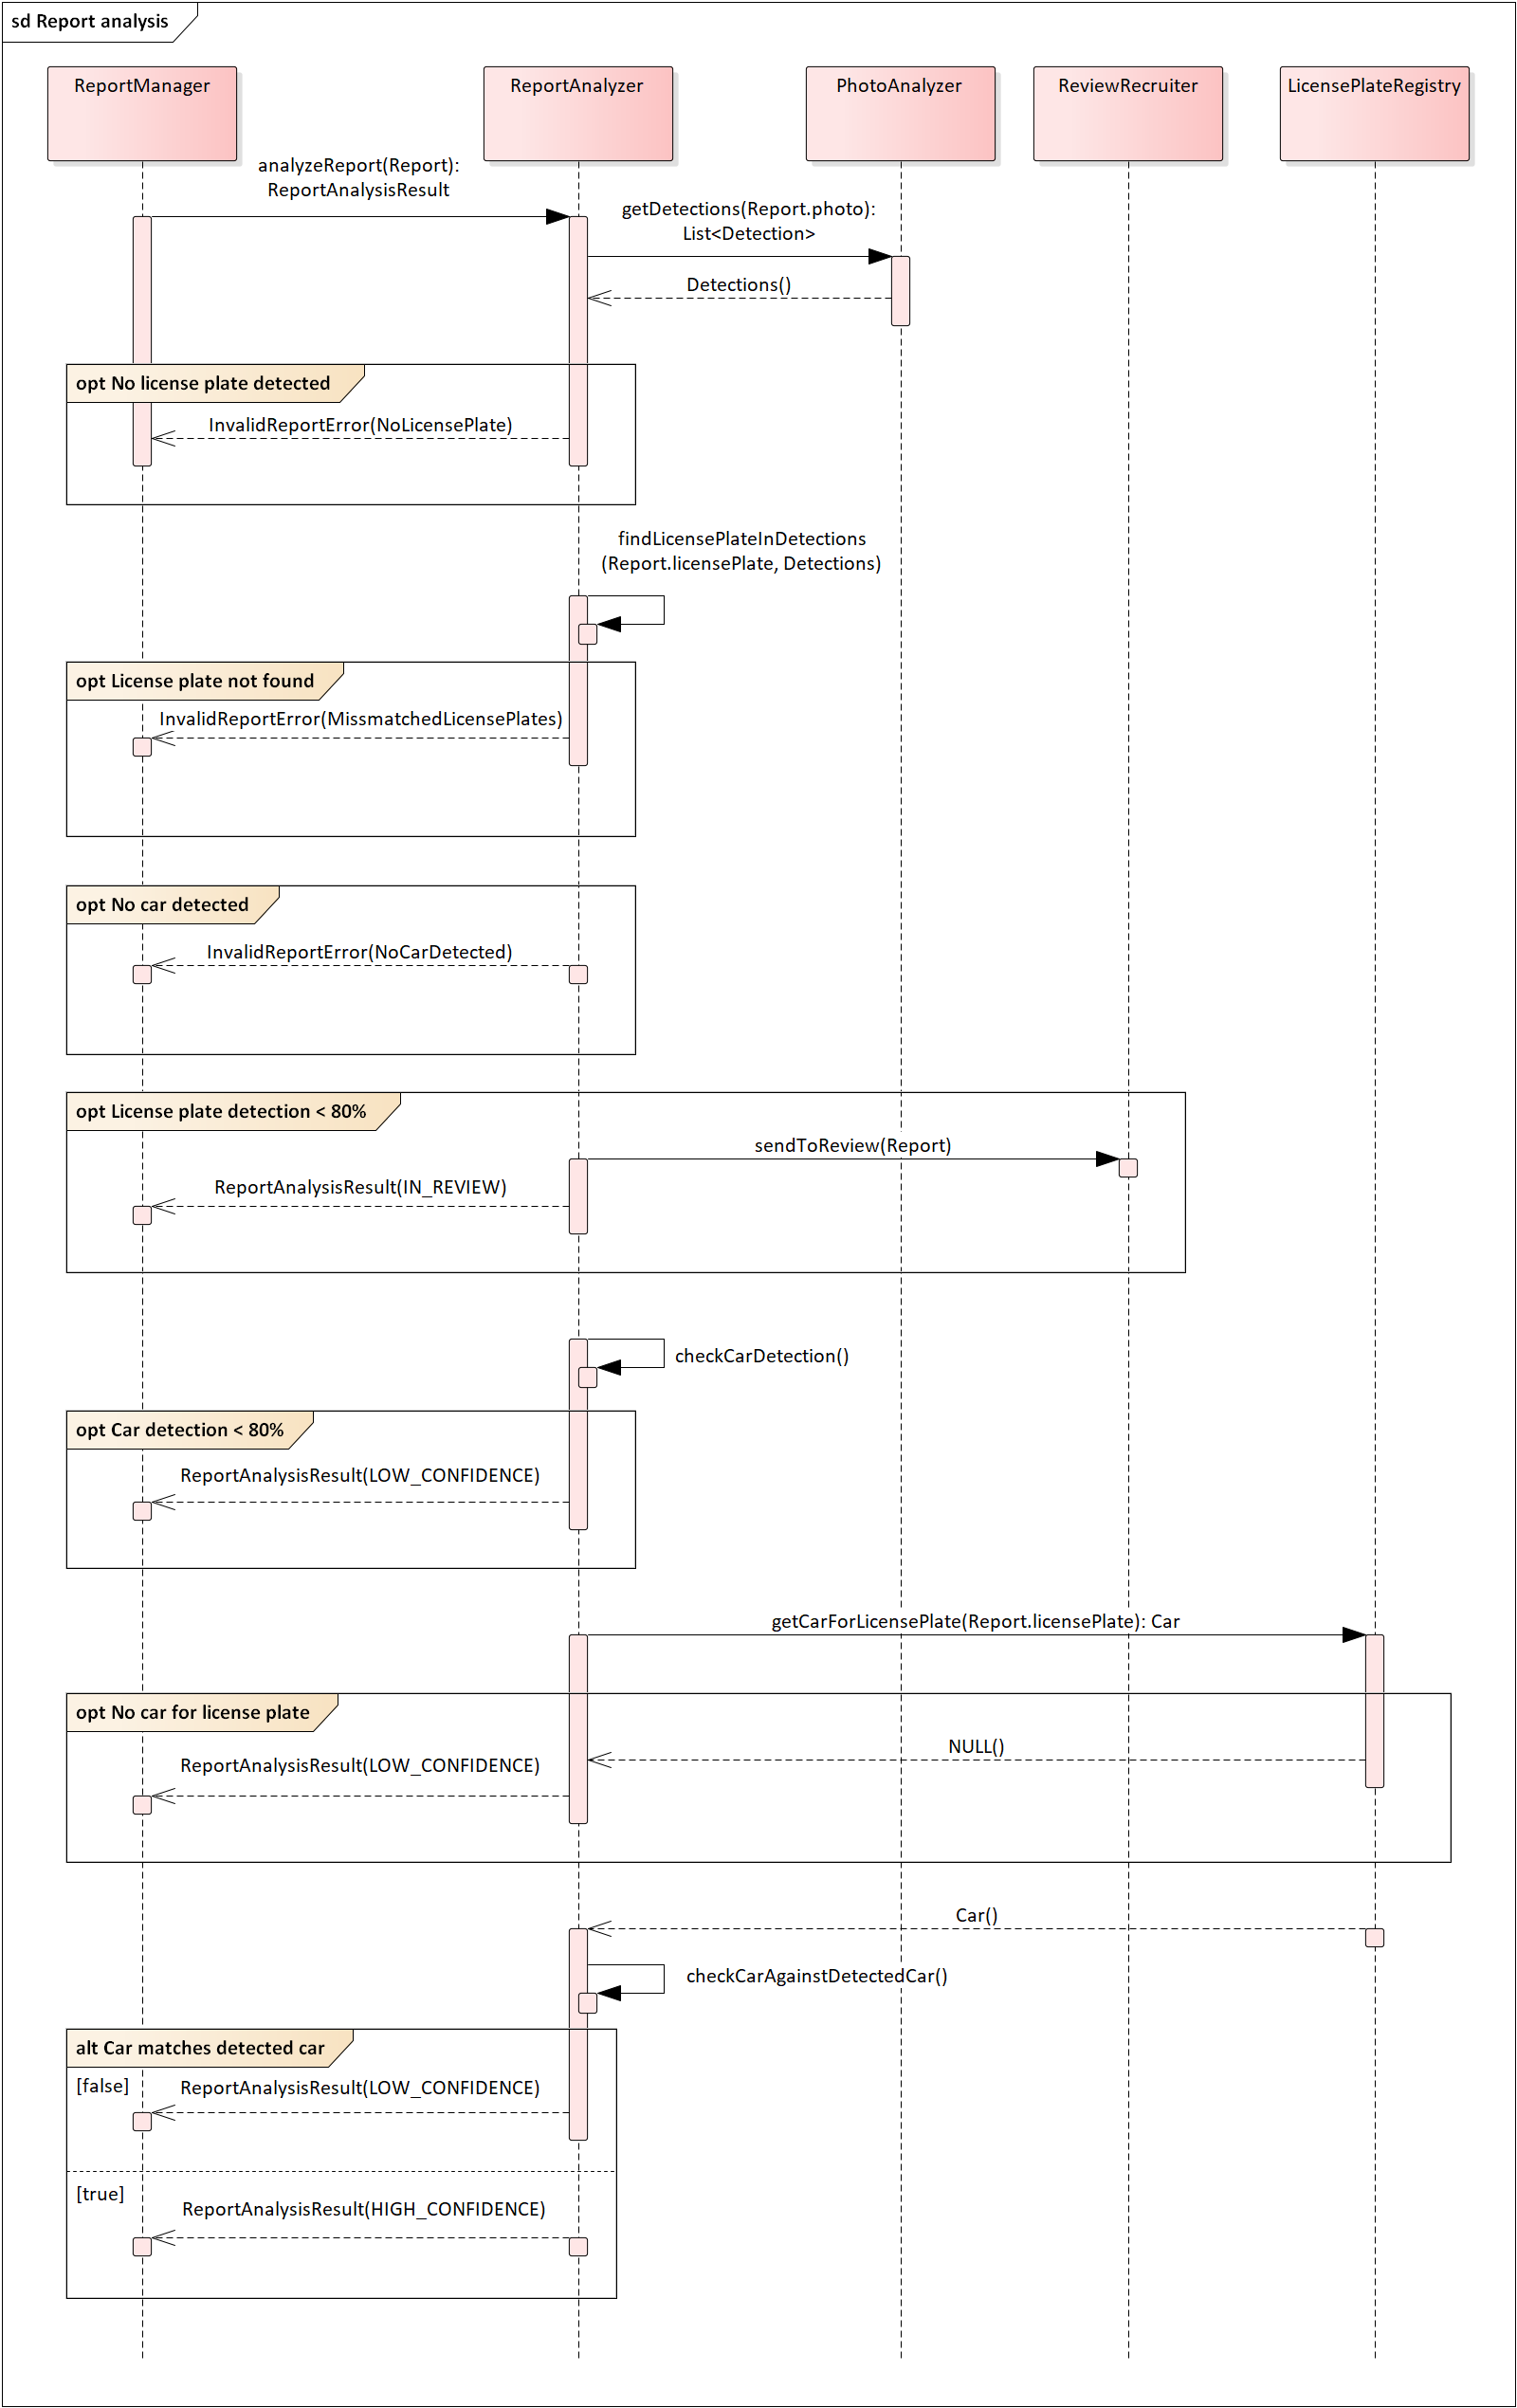
\includegraphics[width=0.9\textwidth]{Images/architectural-design/Sequence/4-Report analysis.png}}
    \caption{\label{fig:sequence-report-analysis}Sequence diagram - Report analysis.}
\end{figure}

\subsubsection{Review recruitment}
The recruitment process is simple. The ReviewRecruiter gets the list of users from the UserRepository, then selects the suitable users from this list. A notification is enqueued for each user in the NotificationQueue.

\begin{figure}[H]
    \centering
    \fbox{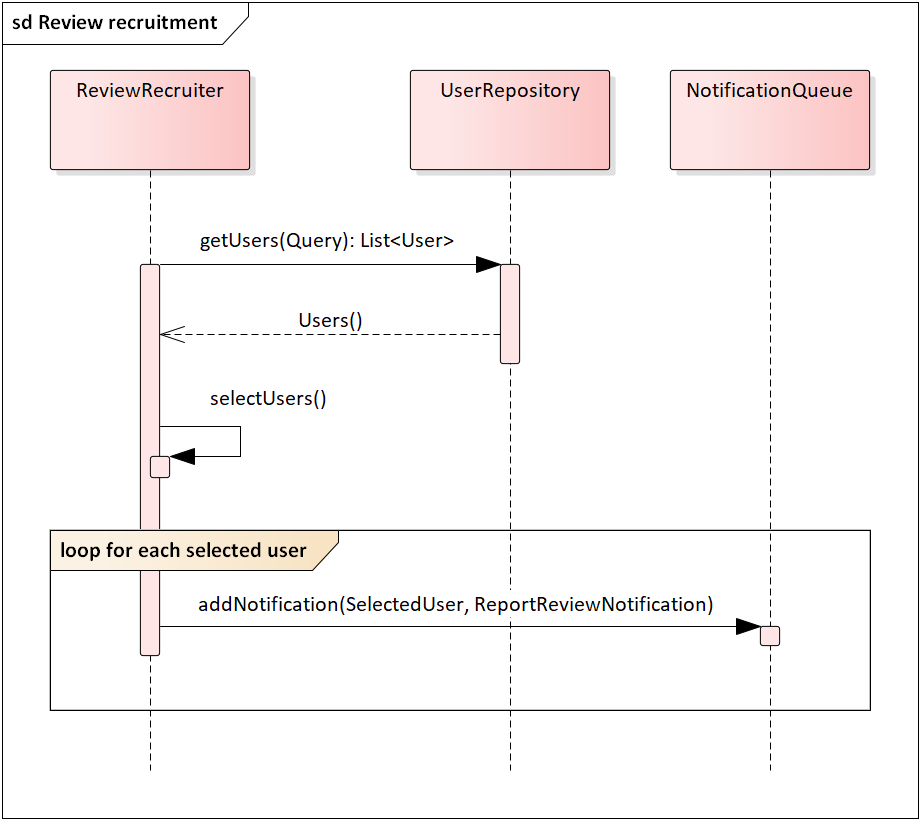
\includegraphics[width=0.95\textwidth]{Images/architectural-design/Sequence/5-Review recruitment.png}}
    \caption{\label{fig:sequence-review-recruitment}Sequence diagram - Review recruitment.}
\end{figure}

\subsubsection{Get notifications}
In this sequence, the user asks for their pending notifications.
The NotificationService first gets the user from the UserManager and then retrieves their pending notifications from the NotificationQueue.

\begin{figure}[H]
    \centering
    \fbox{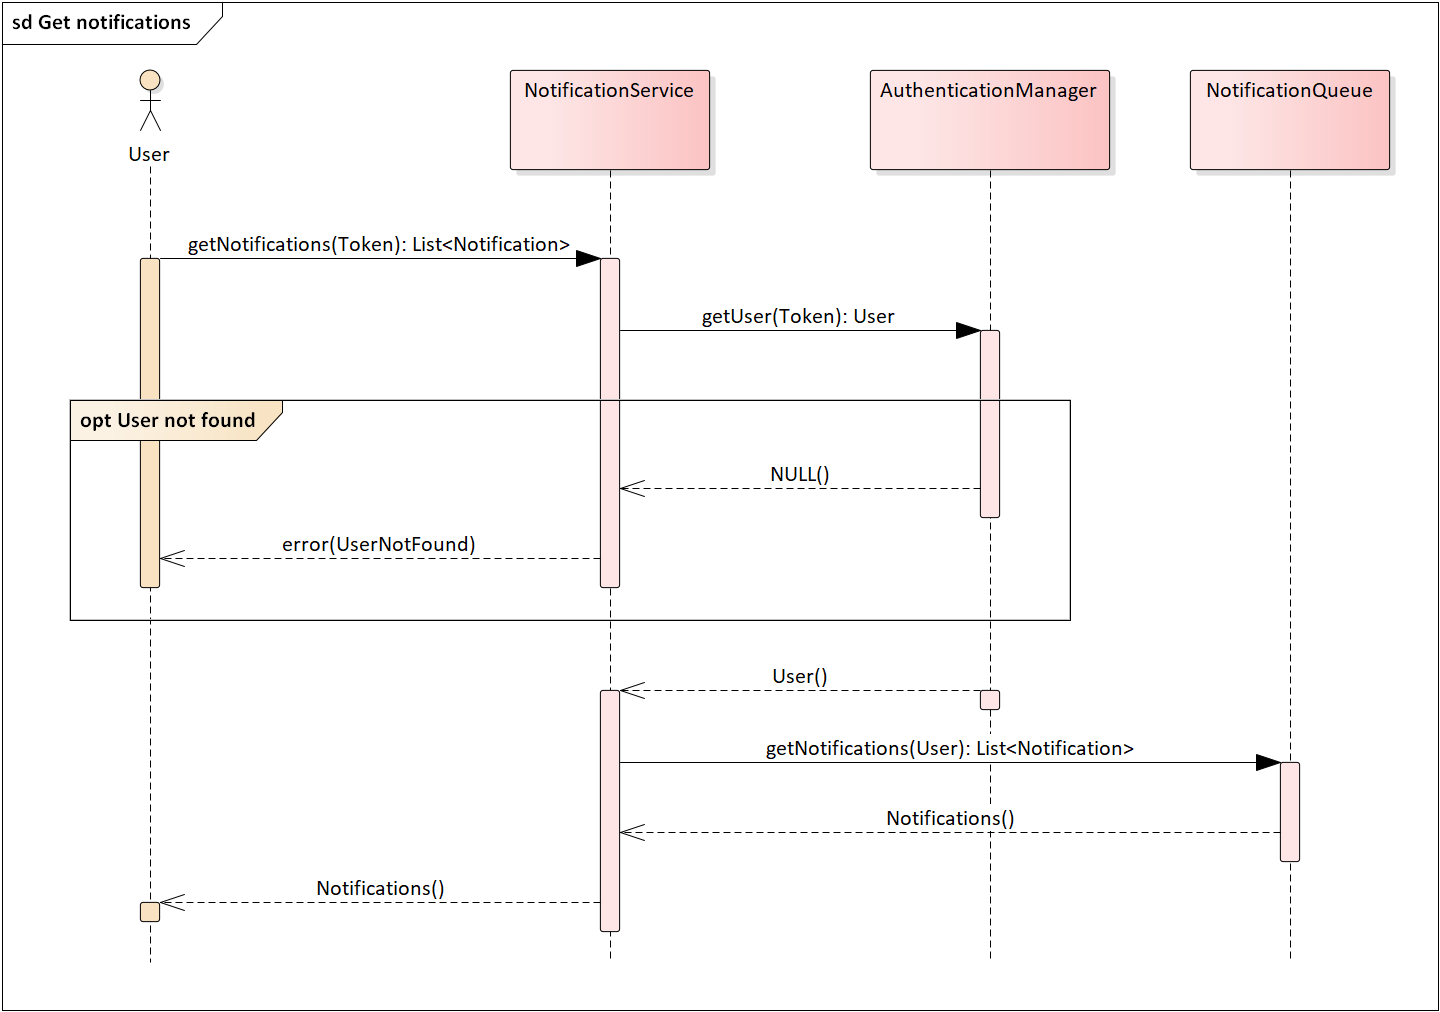
\includegraphics[width=0.95\textwidth]{Images/architectural-design/Sequence/6-Get notifications.png}}
    \caption{\label{fig:sequence-get-notifications}Sequence diagram - Get notifications.}
\end{figure}

\subsubsection{Review submission}
When the user submits a review, the ReportReviewService receives the request and passes the review to the ReviewManager. The ReviewManager stores the review via the ReviewRepository and checks whether the amount of reviews is higher or equal to the decision threshold. If this is not the case then the sequence ends returning an ok code to the user. Otherwise, the report is retrieved from the ReportRepository and is submitted to the ReviewManager along with its review match percentage. Then the ReviewManager interacts with the ReportAnalyzer and the ReportRepository to classify the report as valid or invalid and save the result. An ok code is returned to the user.

\begin{figure}[H]
    \centering
    \fbox{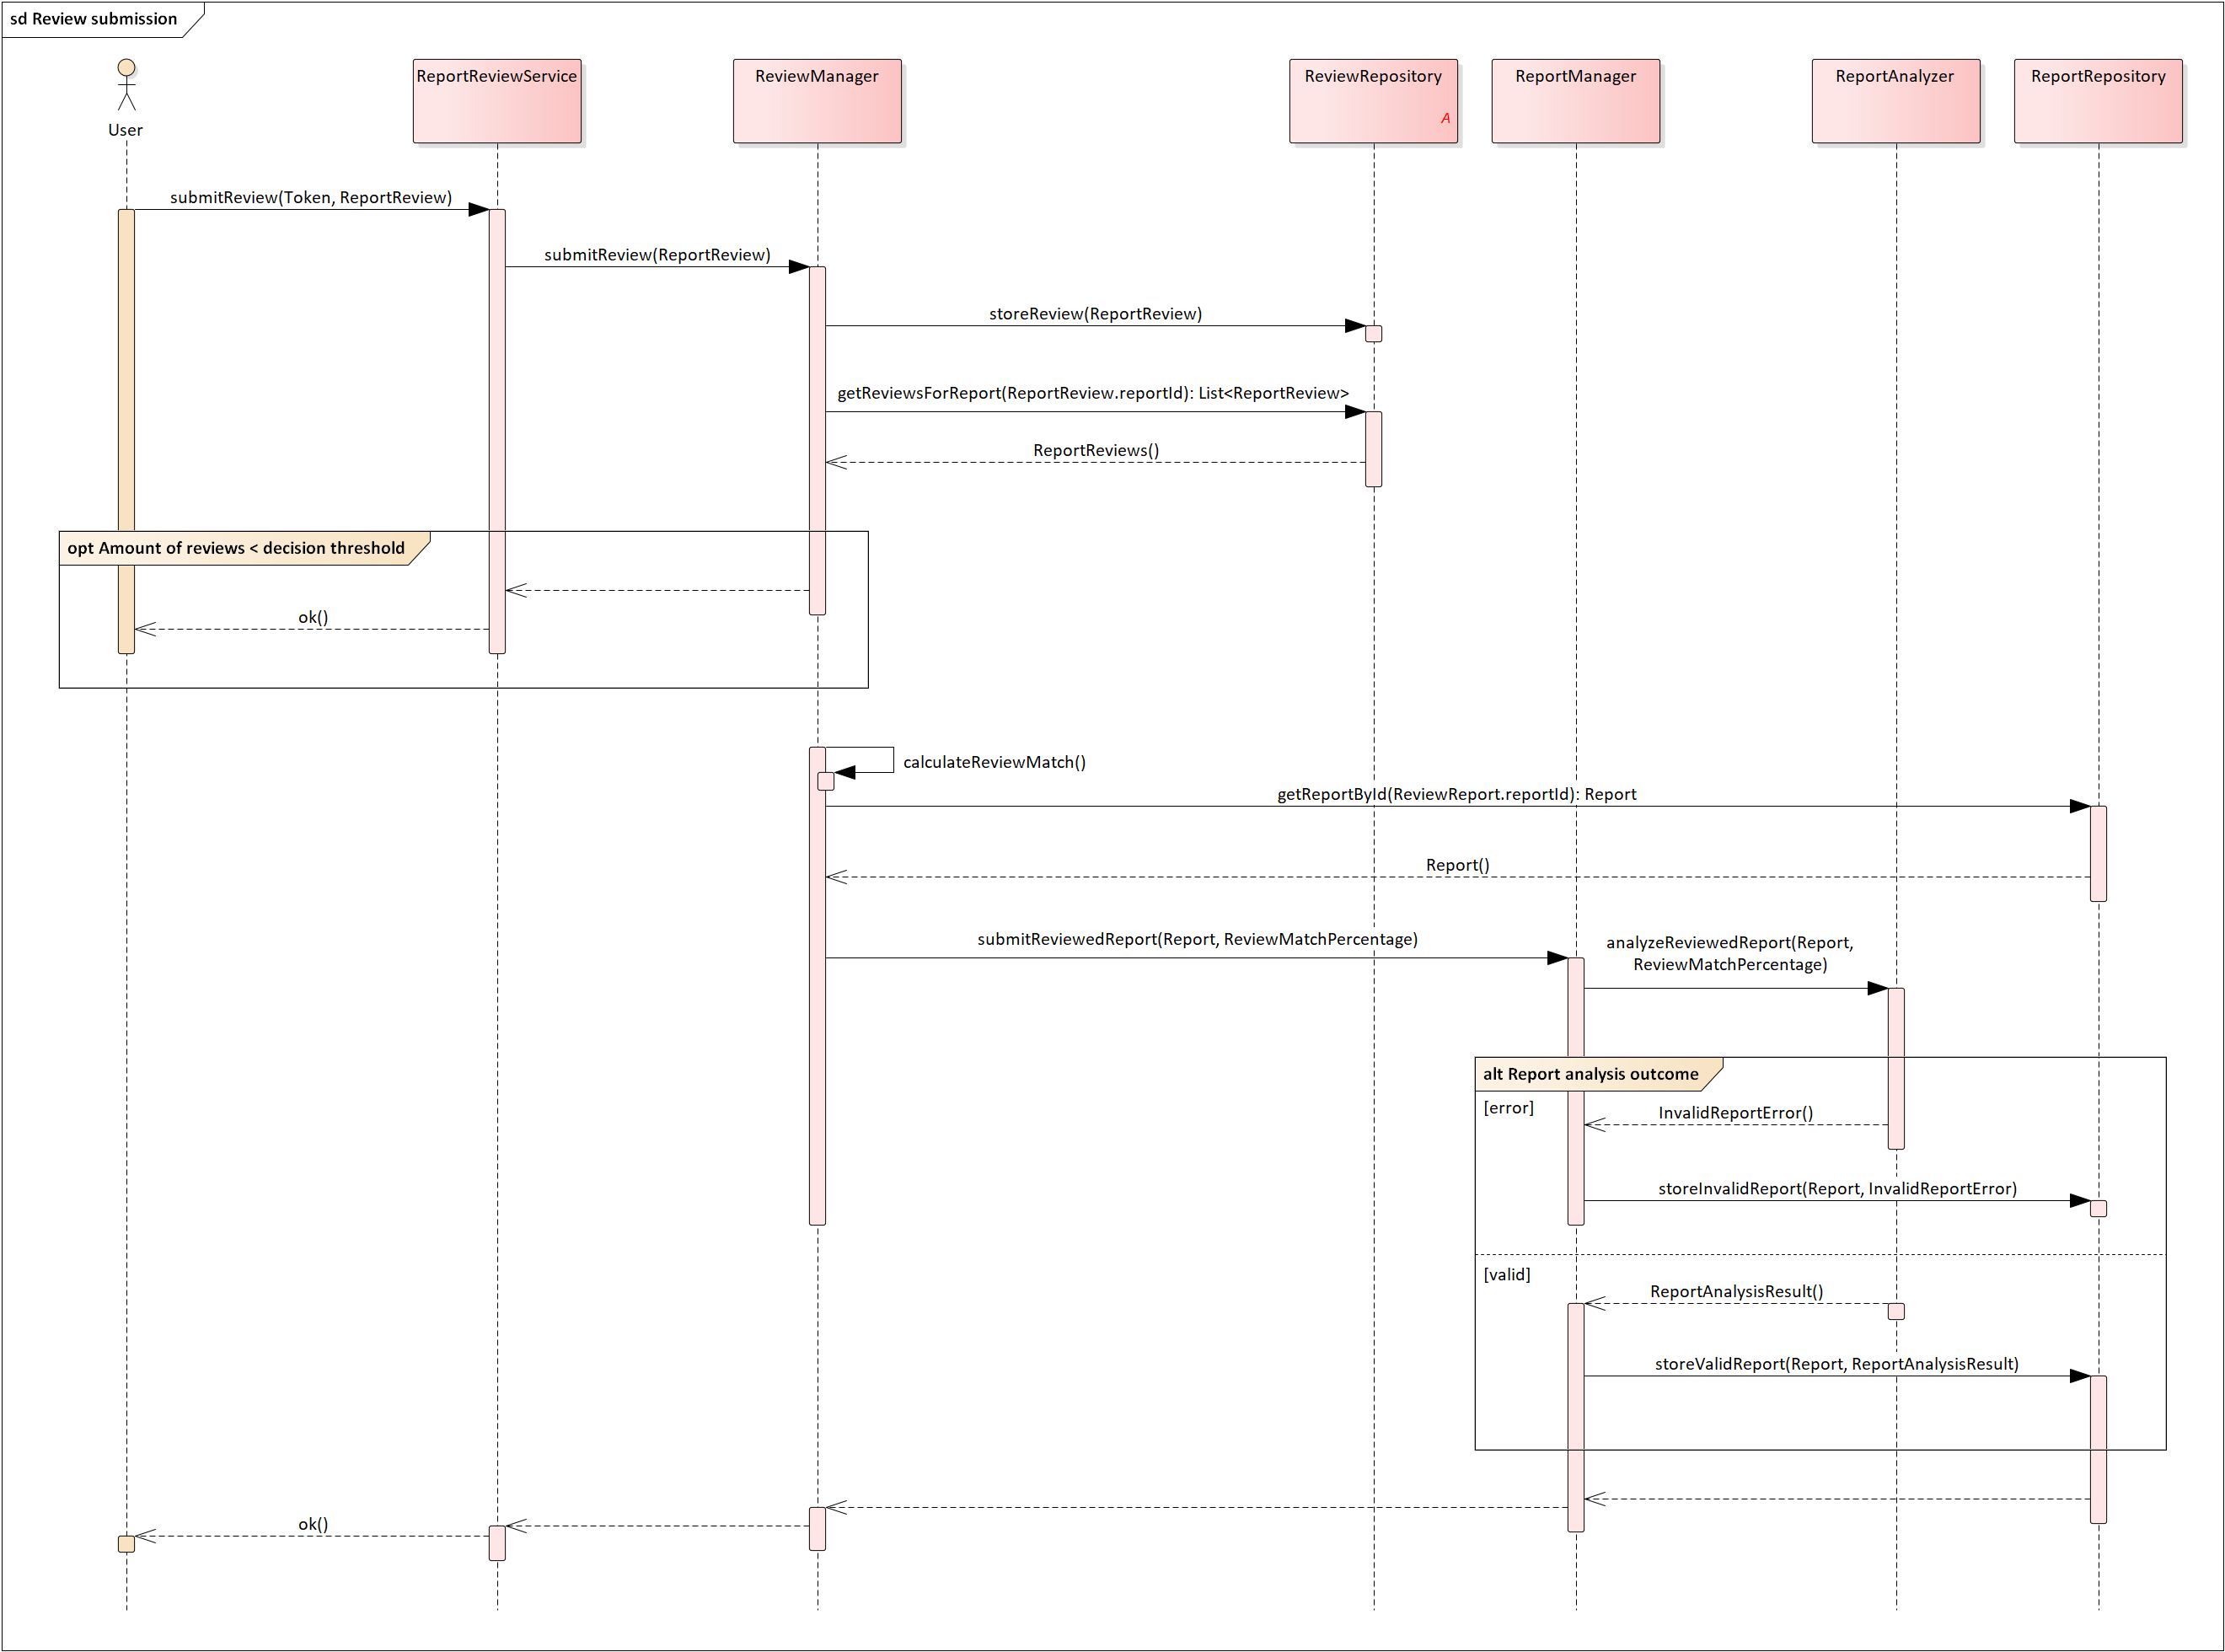
\includegraphics[angle=-90, origin=c, width=0.98\textwidth]{Images/architectural-design/Sequence/7-Review submission.png}}
    \caption{\label{fig:sequence-review-submission}Sequence diagram - Review submission.}
\end{figure}

\subsubsection{Reviewed report analysis}
This sequence is similar to the report analysis, but the review matching percentage is utilized to decide whether the report is invalid or low-confidence at the beginning of the process. If it's considered neither then it proceeds like the normal analysis.

\begin{figure}[H]
    \centering
    \fbox{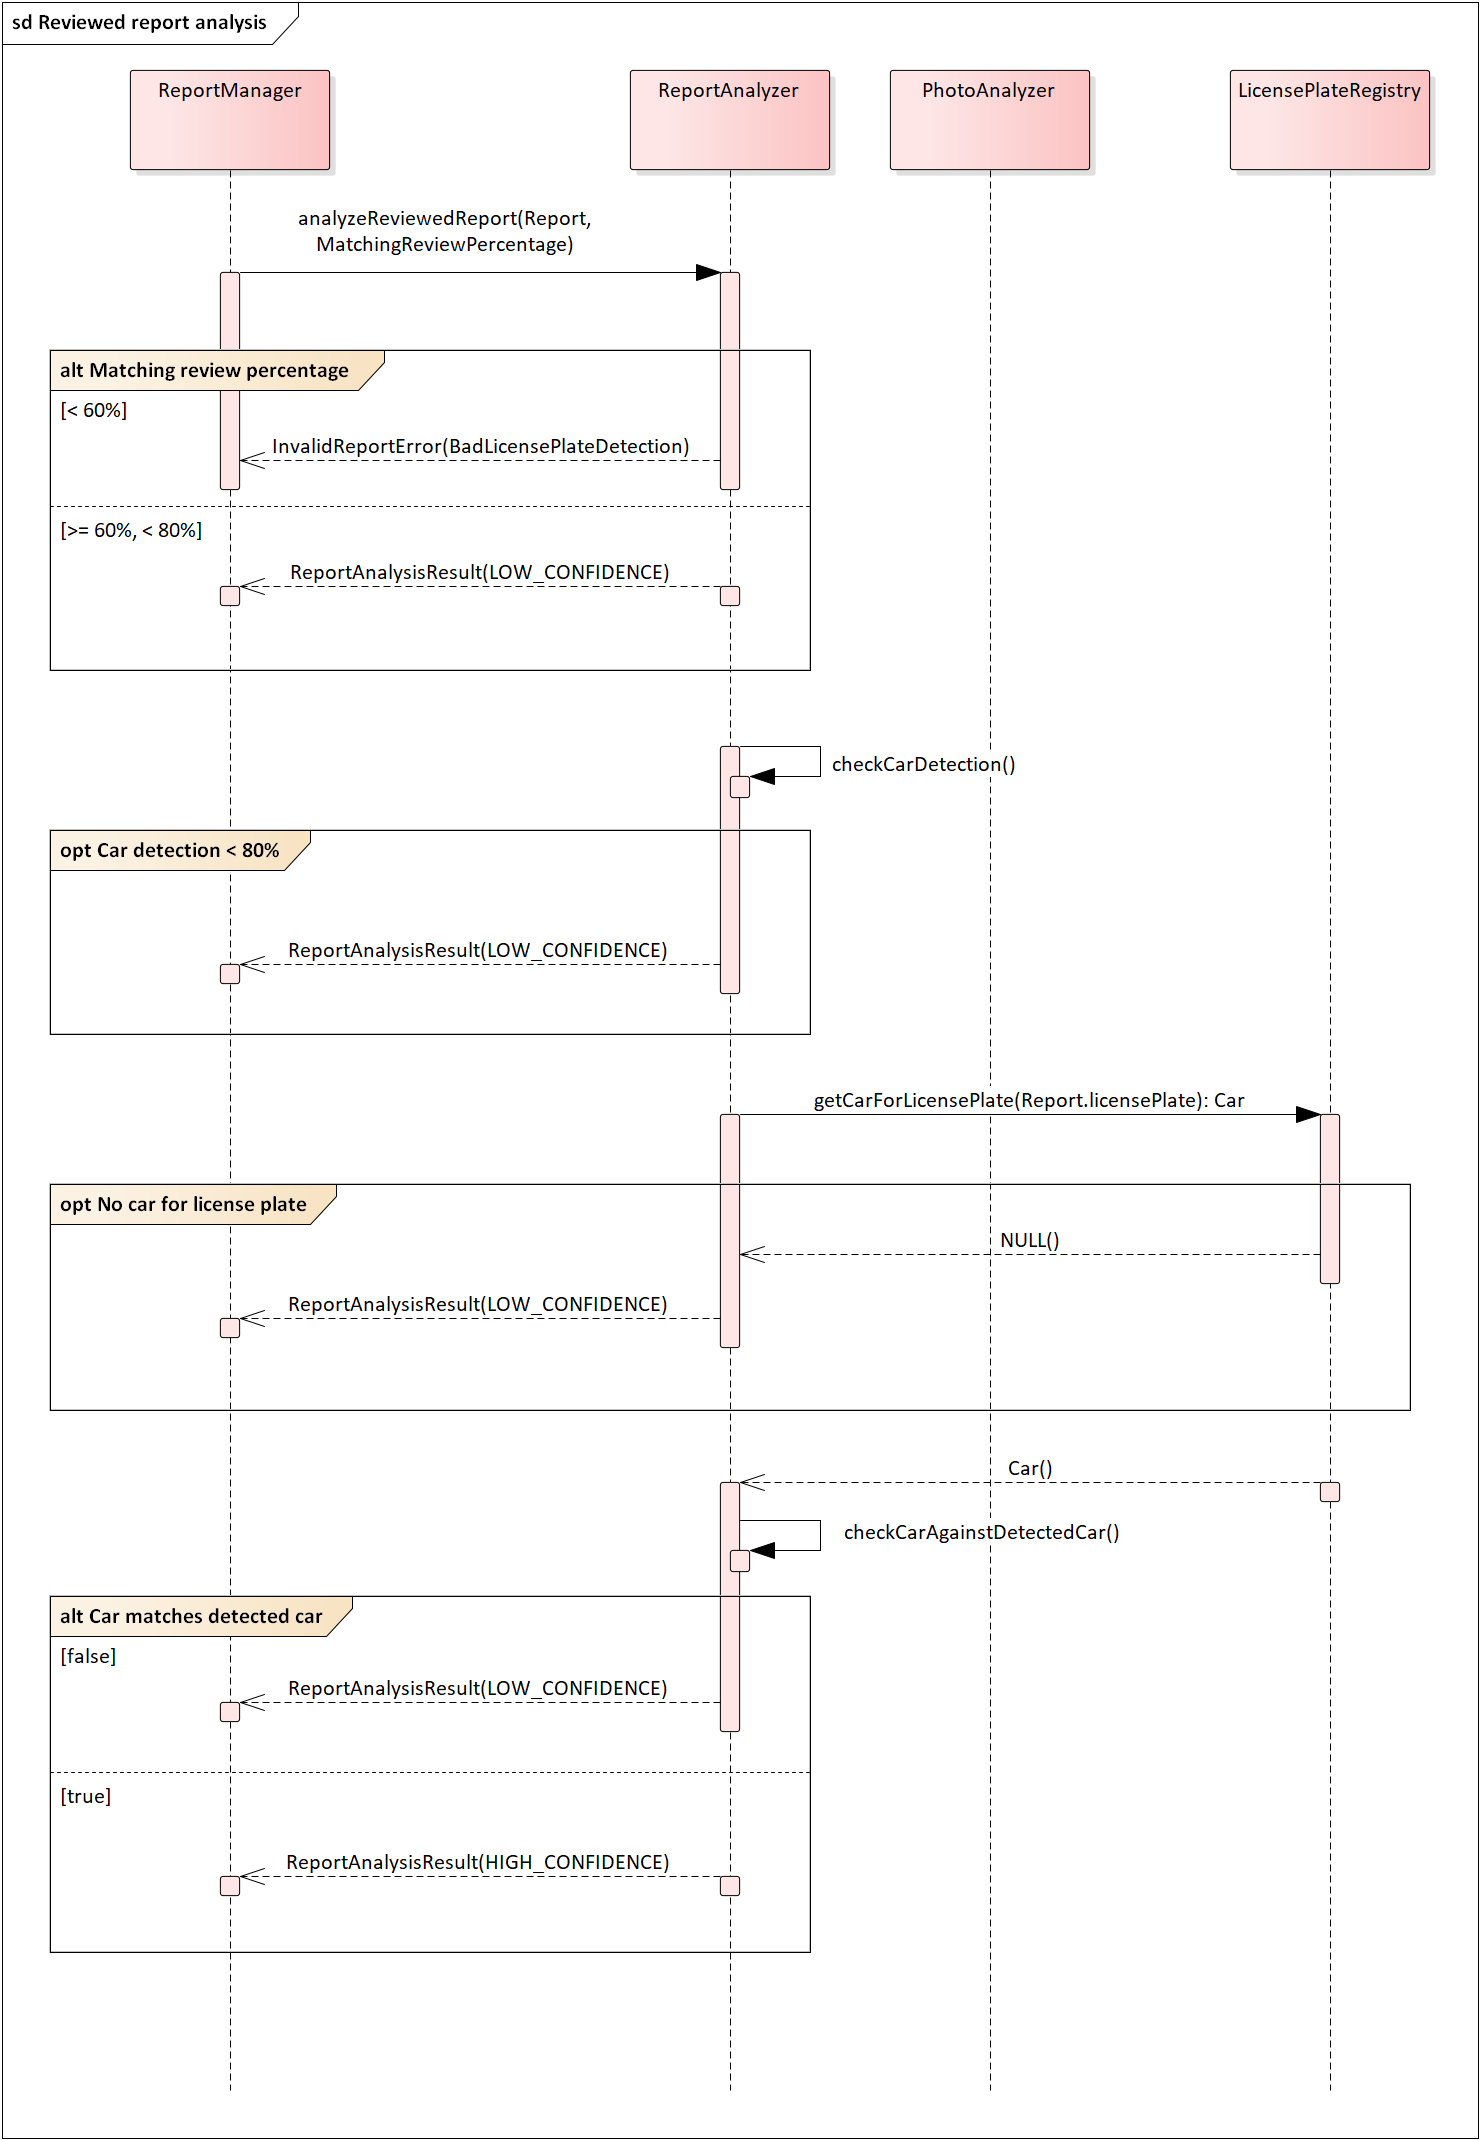
\includegraphics[width=0.88\textwidth]{Images/architectural-design/Sequence/8-Reviewed report analysis.png}}
    \caption{\label{fig:sequence-reviewed-report-analysis}Sequence diagram - Reviewed report analysis.}
\end{figure}

\subsubsection{Get reports}
The ReportService handles the request and asks the ReportsManager for the reports. The ReportManager retrieves the reports from the ReportRepository and interacts with the TicketingSystem to check if the reports have related tickets. Afterwards, sensitive information is removed from the report and a list of reports with partial information is returned to the user.

\begin{figure}[H]
    \centering
    \fbox{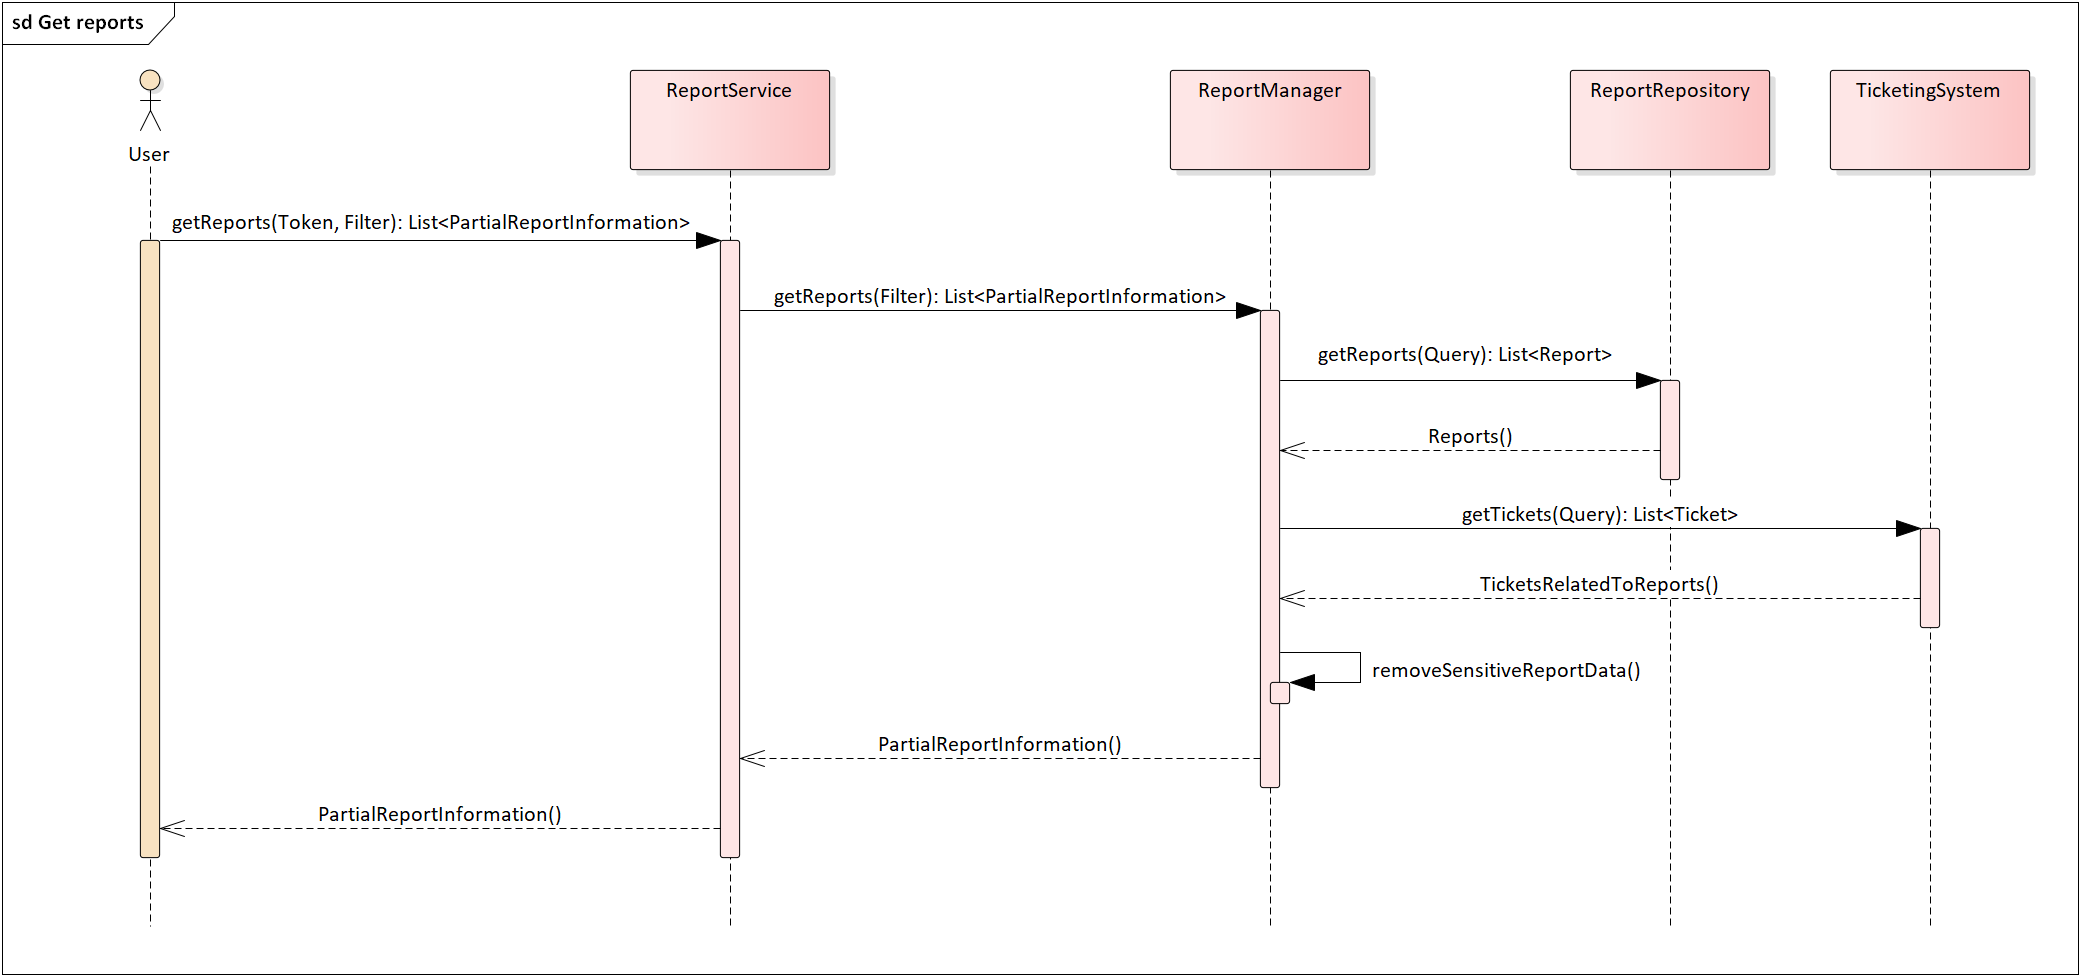
\includegraphics[angle=-90, origin=c, width=0.58\textwidth]{Images/architectural-design/Sequence/9-Get reports.png}}
    \caption{\label{fig:sequence-get-reports}Sequence diagram - Get reports.}
\end{figure}


\subsubsection{Get full reports}
This process is similar to the previous one, but no information is removed from the report, thus including all photos in the report and the target license plate.

\begin{figure}[H]
    \centering
    \fbox{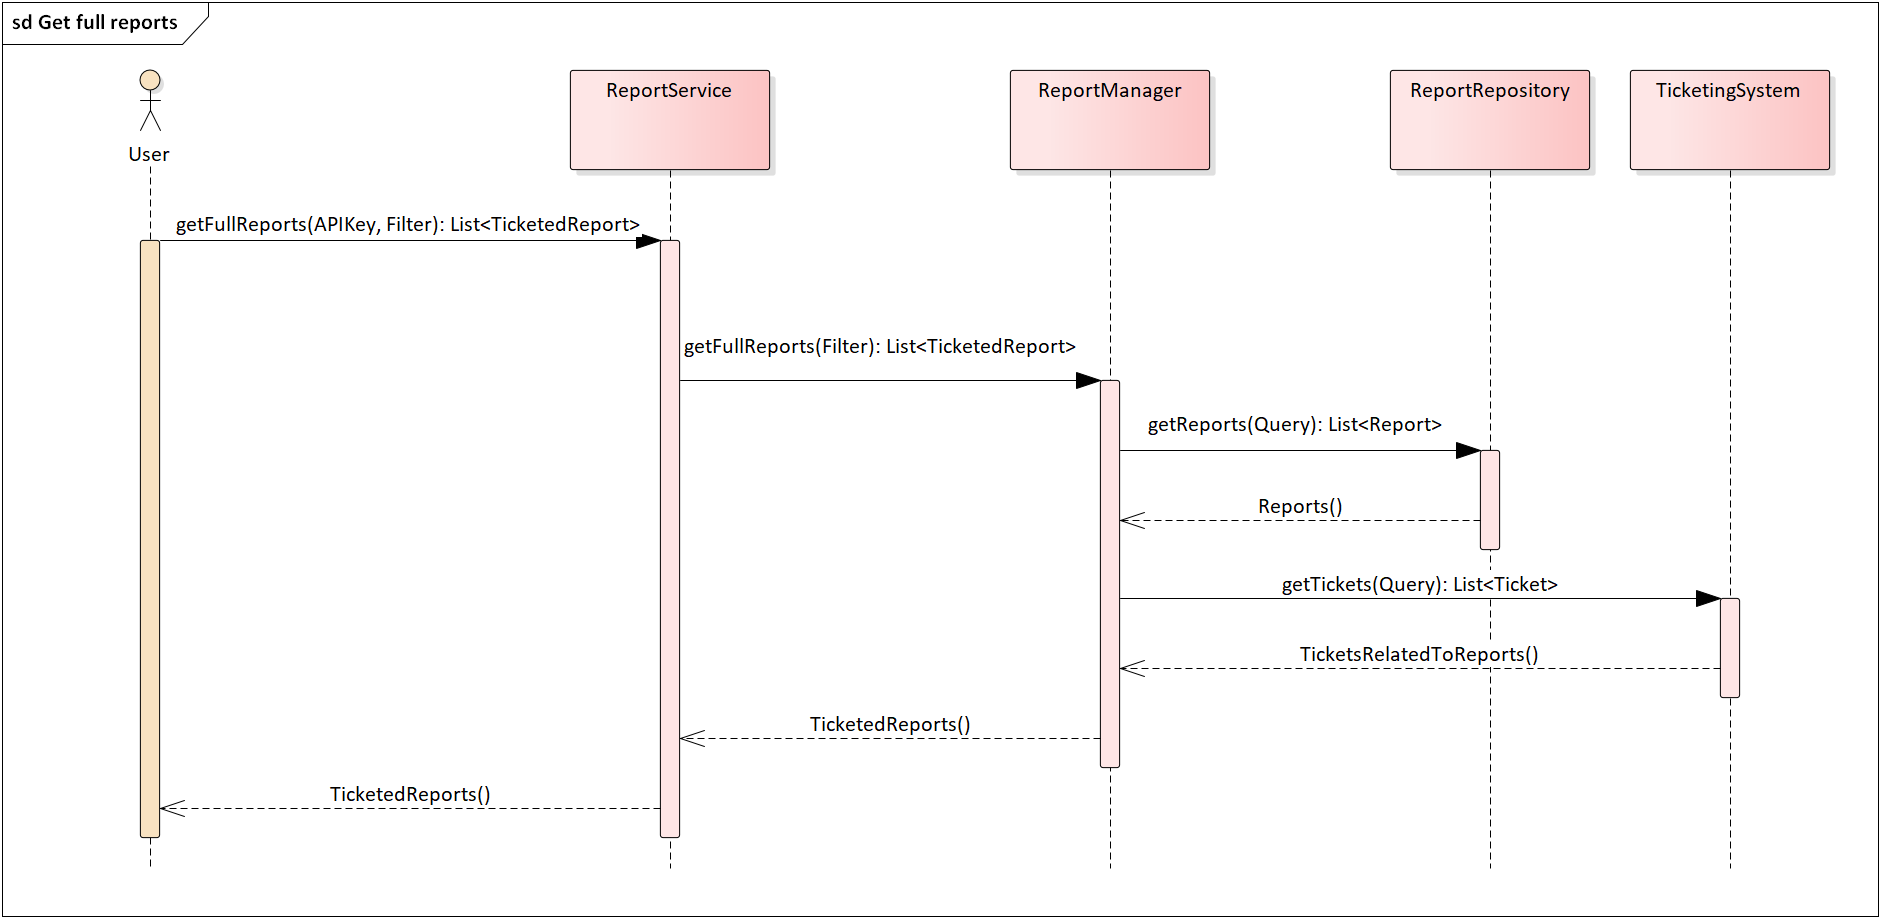
\includegraphics[angle=-90, origin=c, width=0.63\textwidth]{Images/architectural-design/Sequence/10-Get full reports.png}}
    \caption{\label{fig:sequence-get-full-reports}Sequence diagram - Get full reports.}
\end{figure}

\subsubsection{Registration}
This is the standard sign up procedure needed for the user to use the mobile application and be able to get a token when logging in. The RegistrationForm is submitted to the server, where the UserManager validates it (valid, non repeated email, secure password) and, if this validation is successful, stores the new user date.

\begin{figure}[H]
    \centering
    \fbox{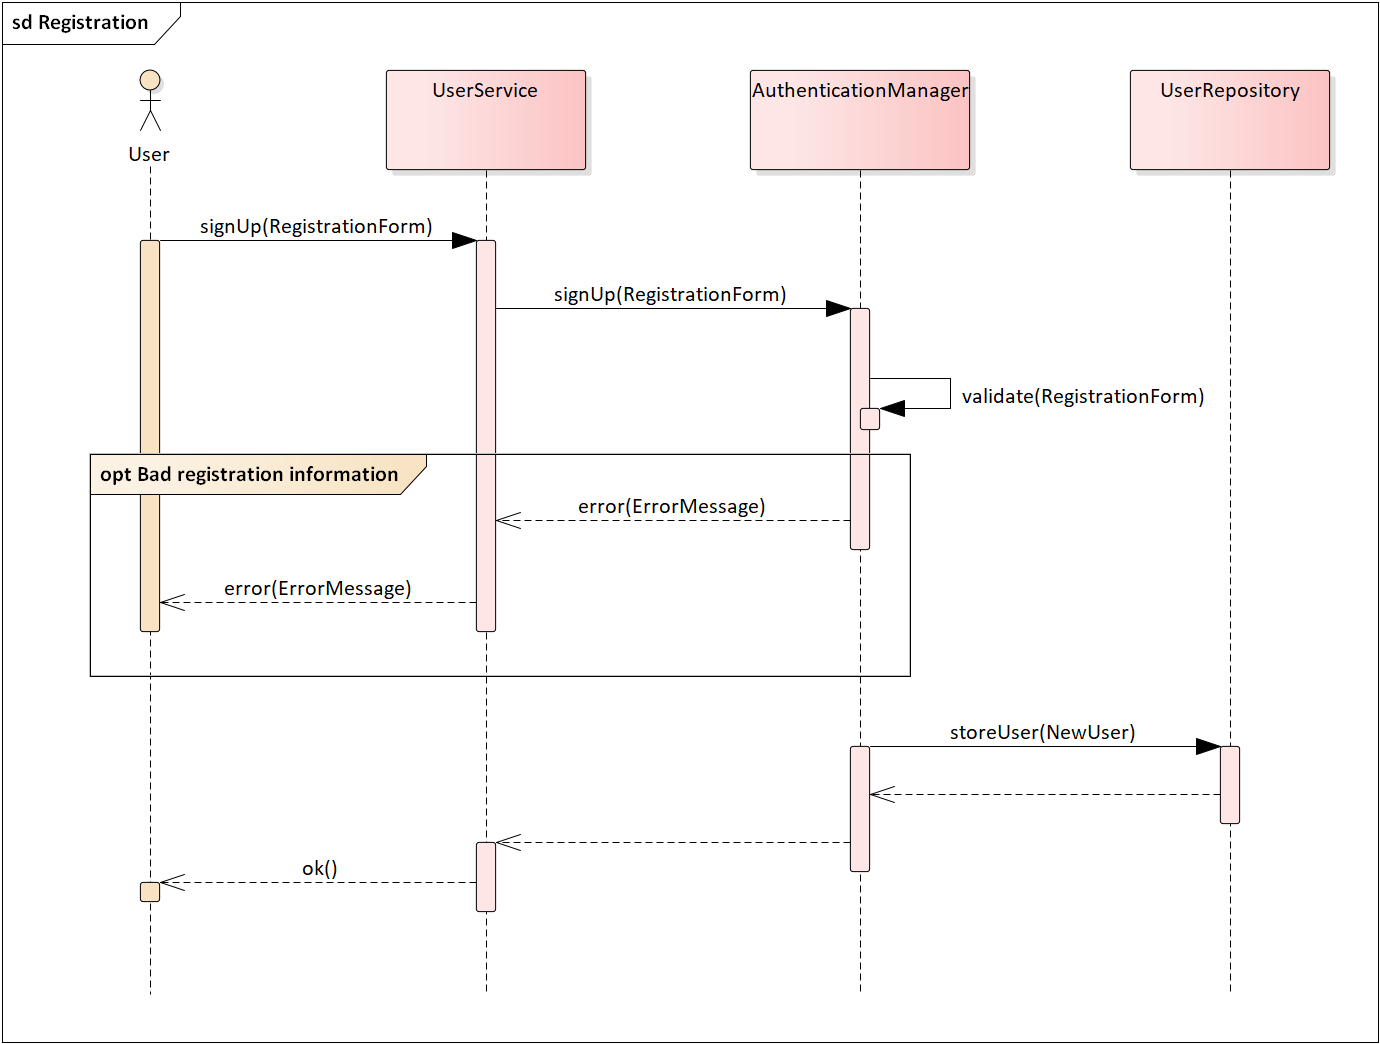
\includegraphics[width=0.95\textwidth]{Images/architectural-design/Sequence/11-Registration.png}}
    \caption{\label{fig:sequence-registration}Sequence diagram - Registration.}
\end{figure}

\subsubsection{Login}
The user enters their email and password, then the server looks for a registered user with that information, if it is found, a token is generated and returned, otherwise an error message is sent.

\begin{figure}[H]
    \centering
    \fbox{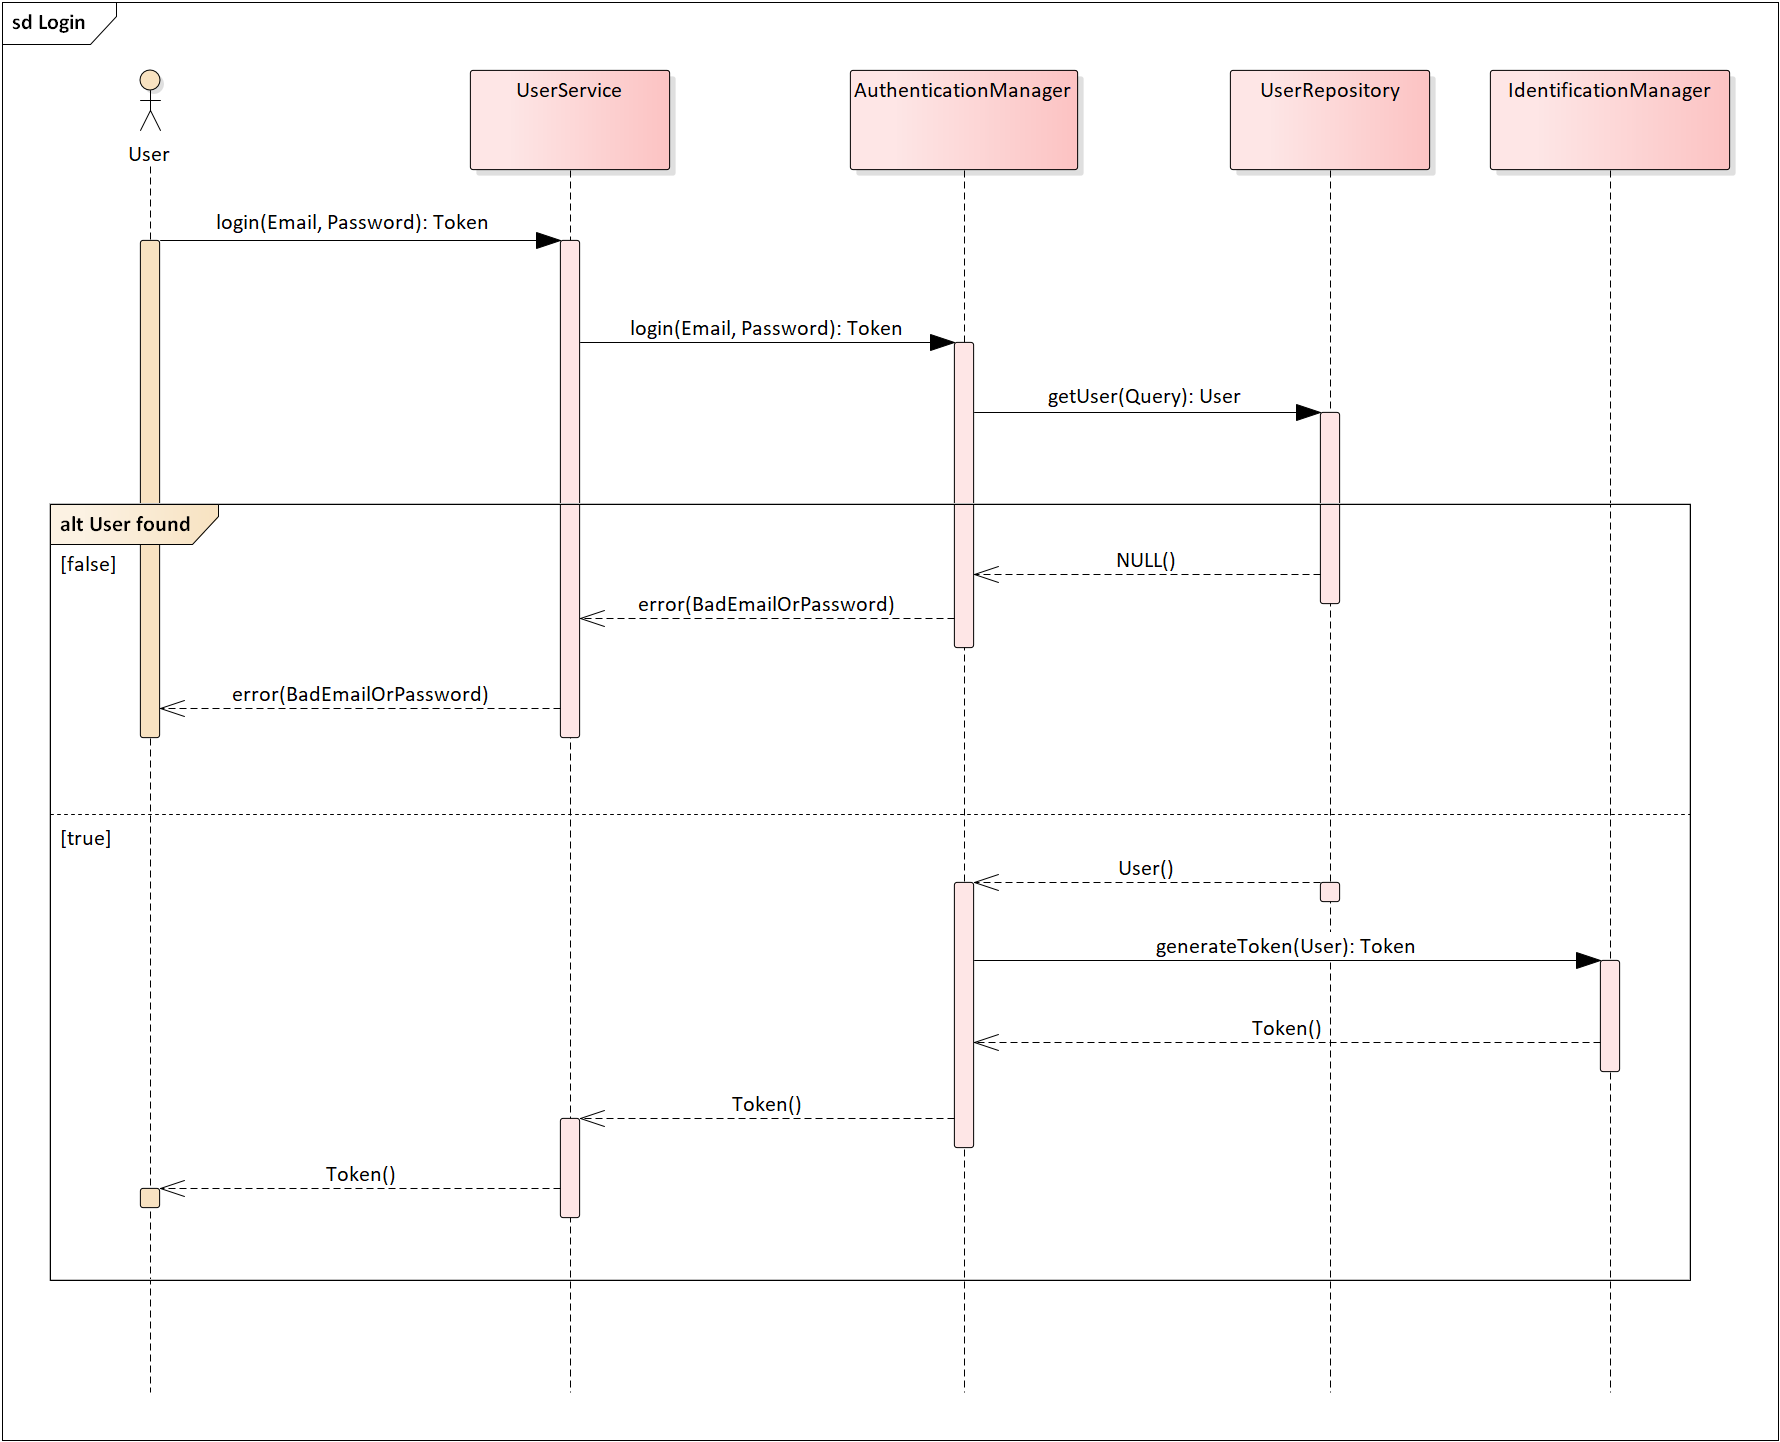
\includegraphics[angle=-90, origin=c, width=0.98\textwidth]{Images/architectural-design/Sequence/12-Login.png}}
    \caption{\label{fig:sequence-registration}Sequence diagram - Login.}
\end{figure}

\subsubsection{Get user information}
The user solicits to obtain their stored information in the system. By looking at the token, the UserManager can query the UserRepository and provide this data if a user is found, otherwise an error message is sent (realistically speaking, this will never fail as the token has to first be verified by the AuthGuard for authorization purposes).

\begin{figure}[H]
    \centering
    \fbox{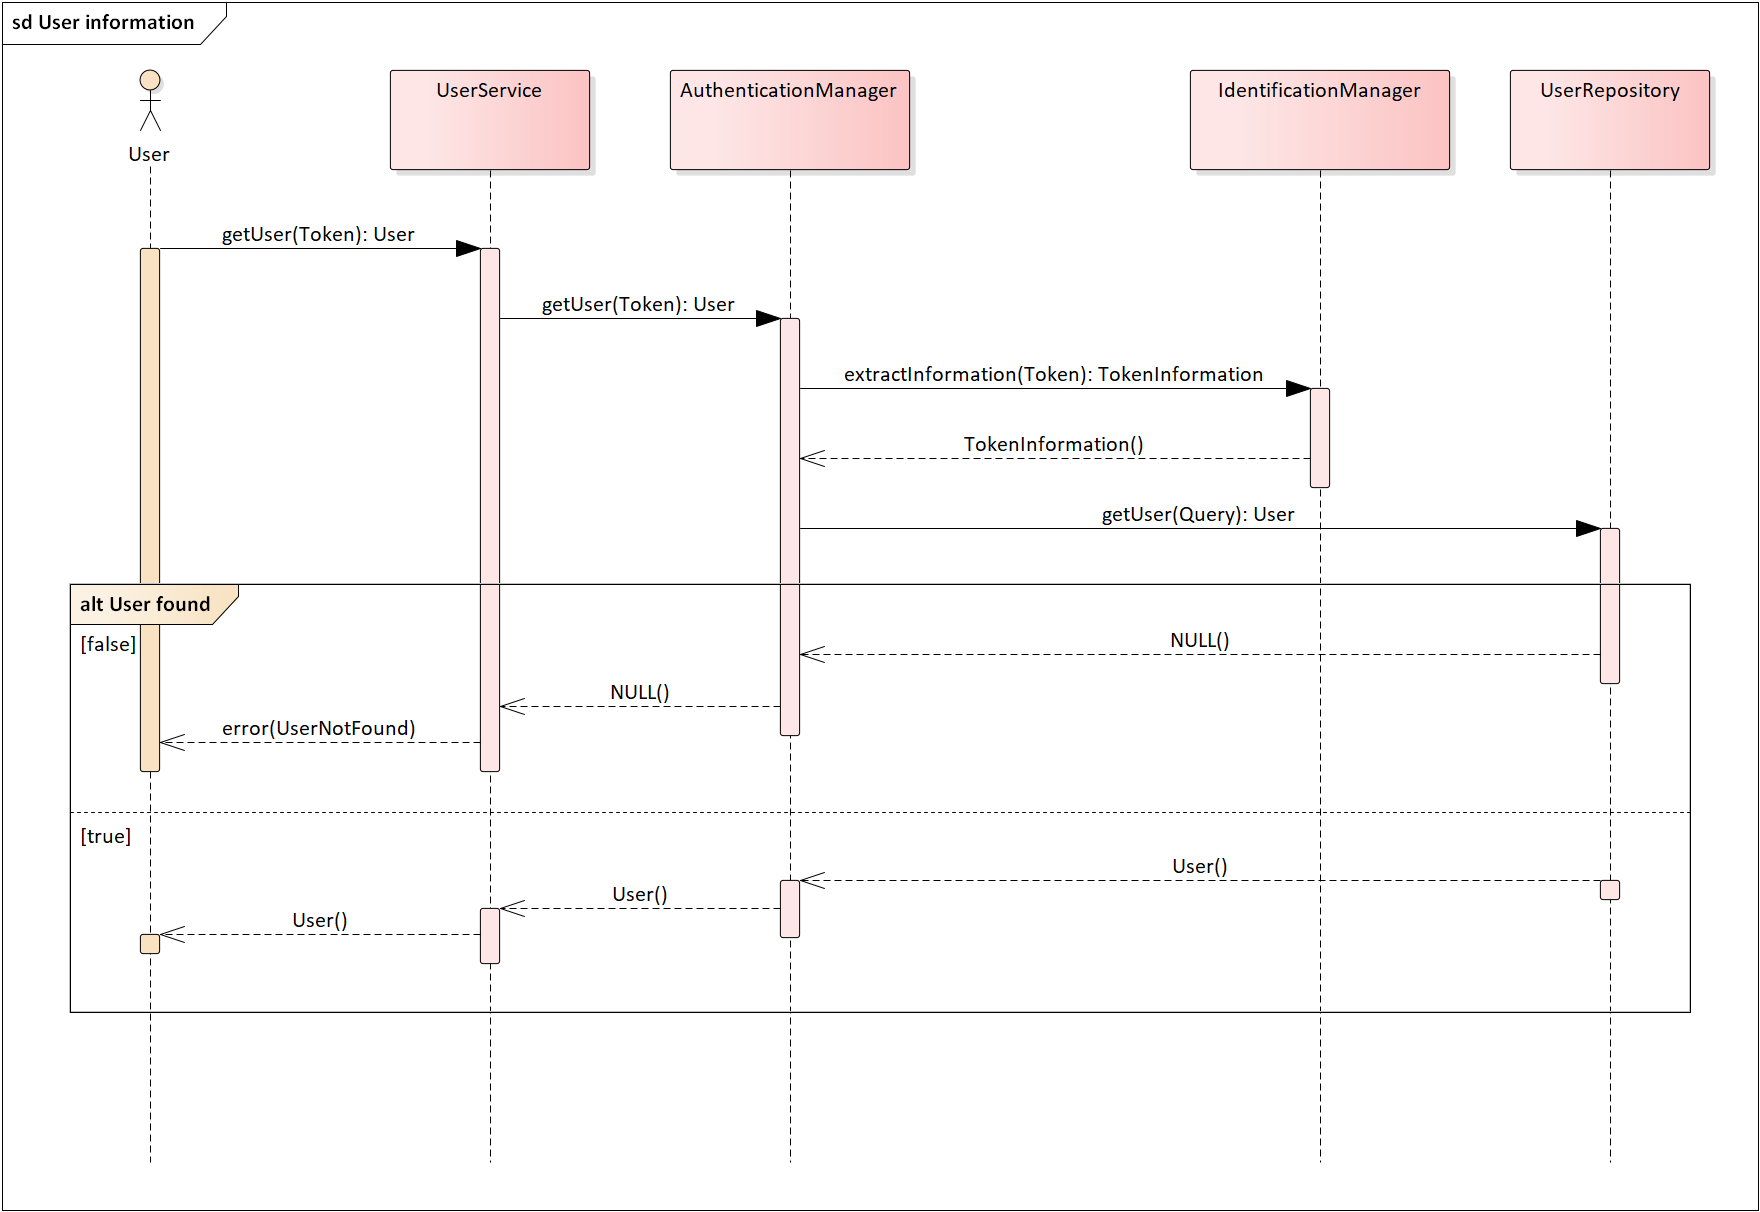
\includegraphics[angle=-90, origin=c, width=0.98\textwidth]{Images/architectural-design/Sequence/13-User information.png}}
    \caption{\label{fig:sequence-user-information}Sequence diagram - Get user information.}
\end{figure}

\subsubsection{Edit user information}
The user submits a form containing the desired information to change in their profile. The UserService looks for the stored User with the given token, if found, the information submitted is validated and if this succeeds the data is modified and stored again in the UserRepository.

\begin{figure}[H]
    \centering
    \fbox{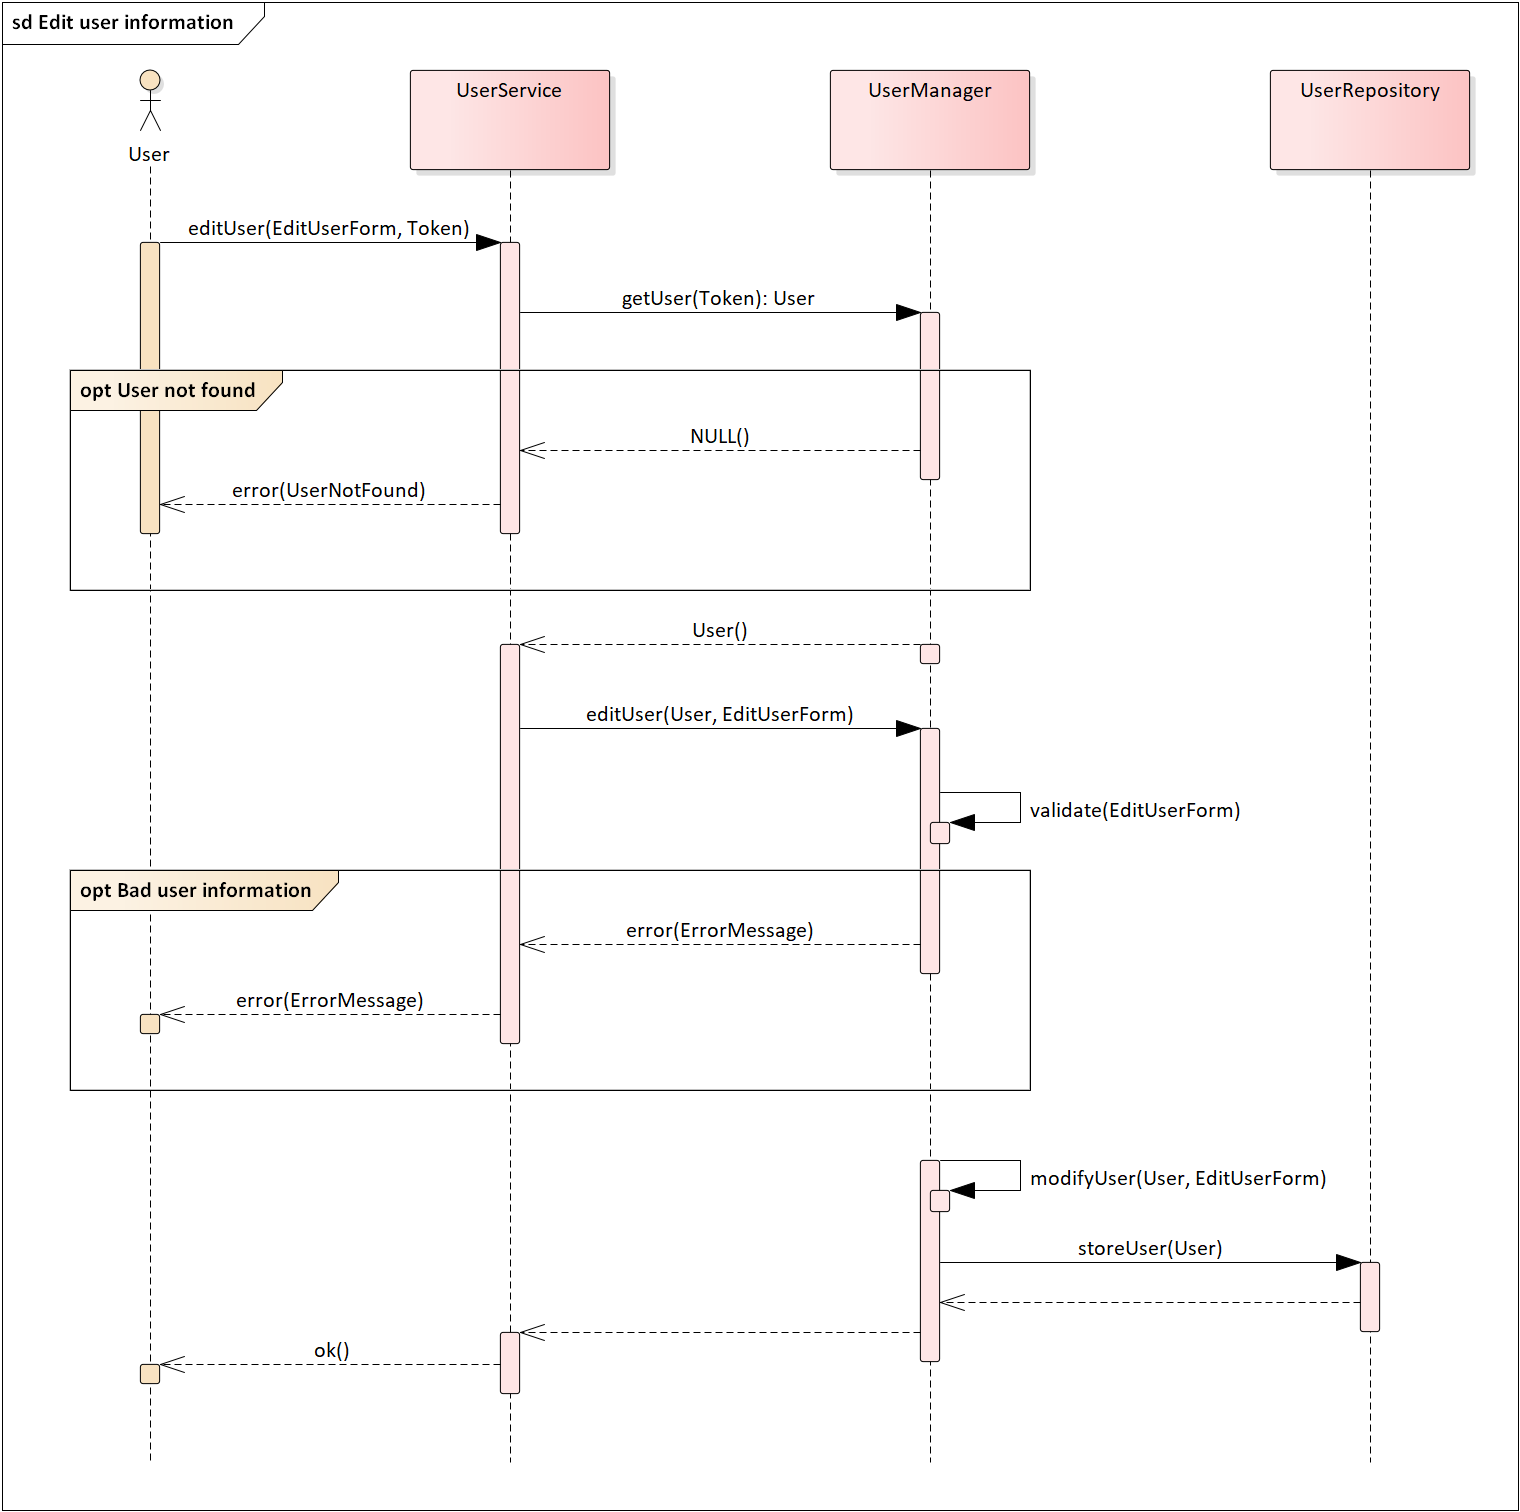
\includegraphics[width=0.98\textwidth]{Images/architectural-design/Sequence/14-Edit user information.png}}
    \caption{\label{fig:sequence-user-information}Sequence diagram - Edit user information.}
\end{figure}

\subsection{Component interfaces}
The interfaces shown in Section~\ref{sub-sect:component-view}  which connect the components internally and expose the public API are detailed here. Each component introduced there is included here, along with the interface it implements. Connections between the interfaces and the component that uses them are not included, as they are already present in the component diagram of Section~\ref{sub-sect:component-view}.

\begin{figure}[H]
    \centering
    \fbox{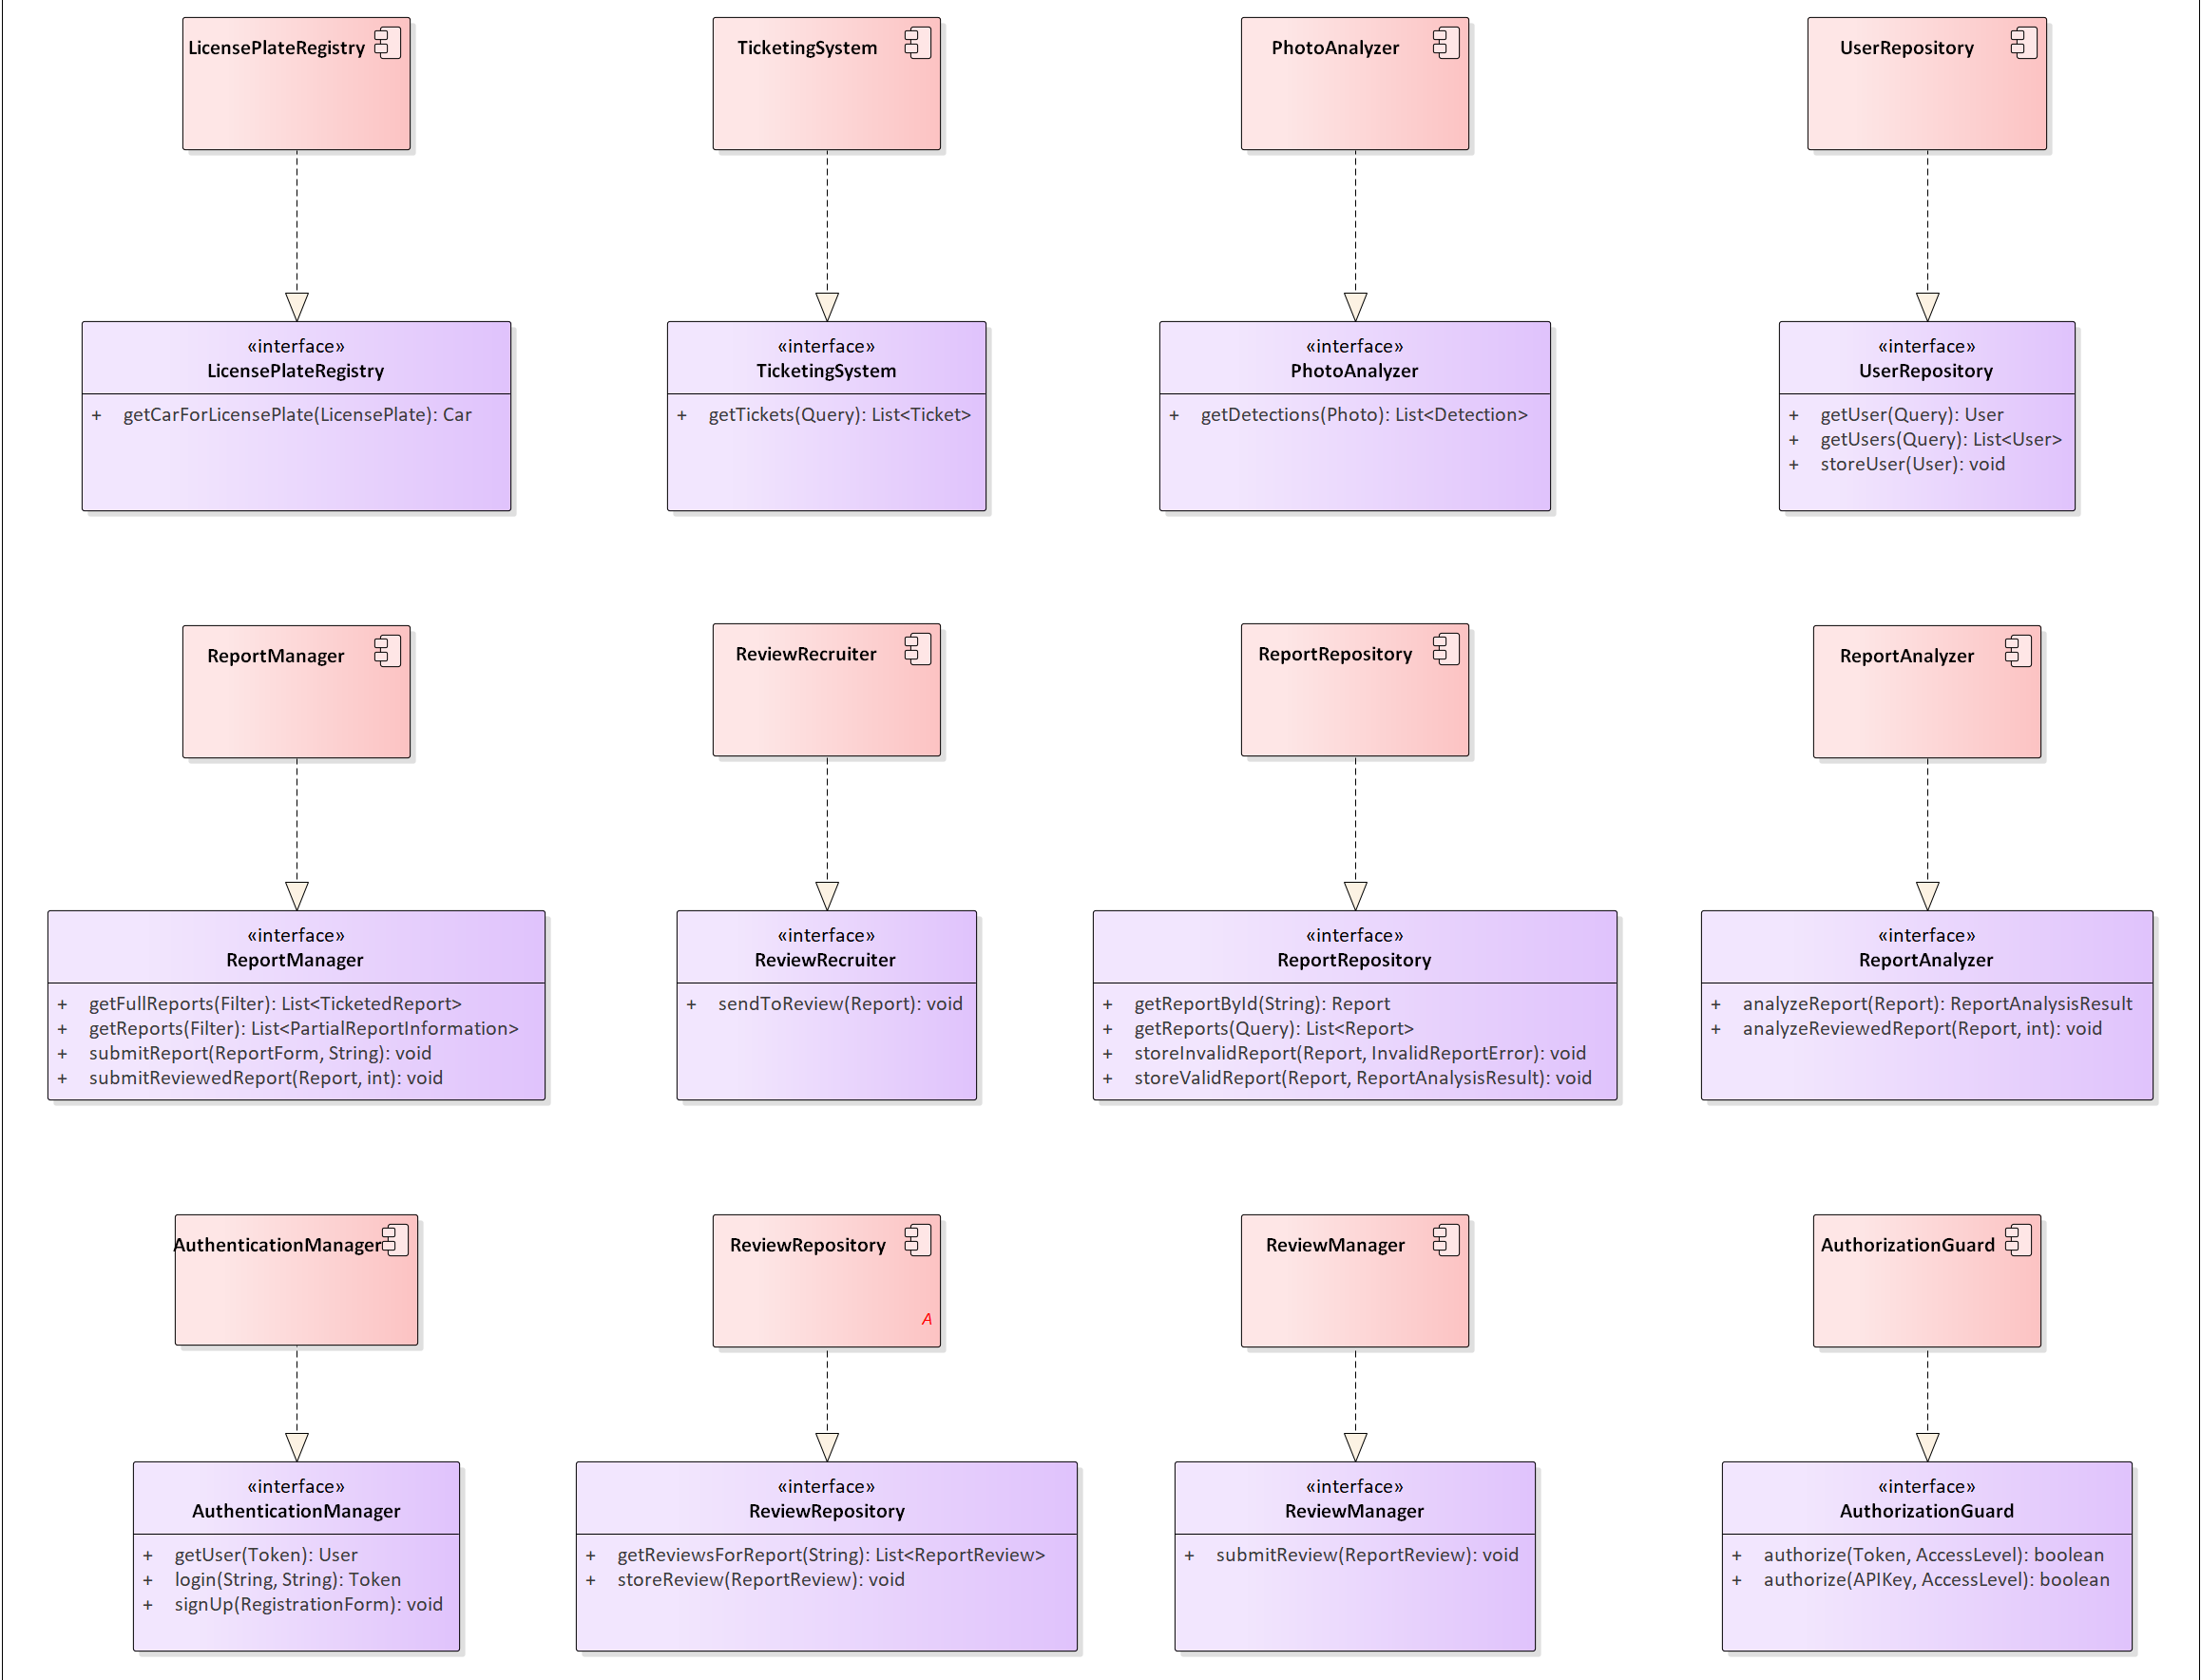
\includegraphics[angle=-90, origin=c, width=0.95\textwidth]{Images/architectural-design/Interfaces 1 of 2.png}}
    \caption{\label{fig:interfaces-1}Component interfaces (1/2).}
\end{figure}

\begin{figure}[H]
    \centering
    \fbox{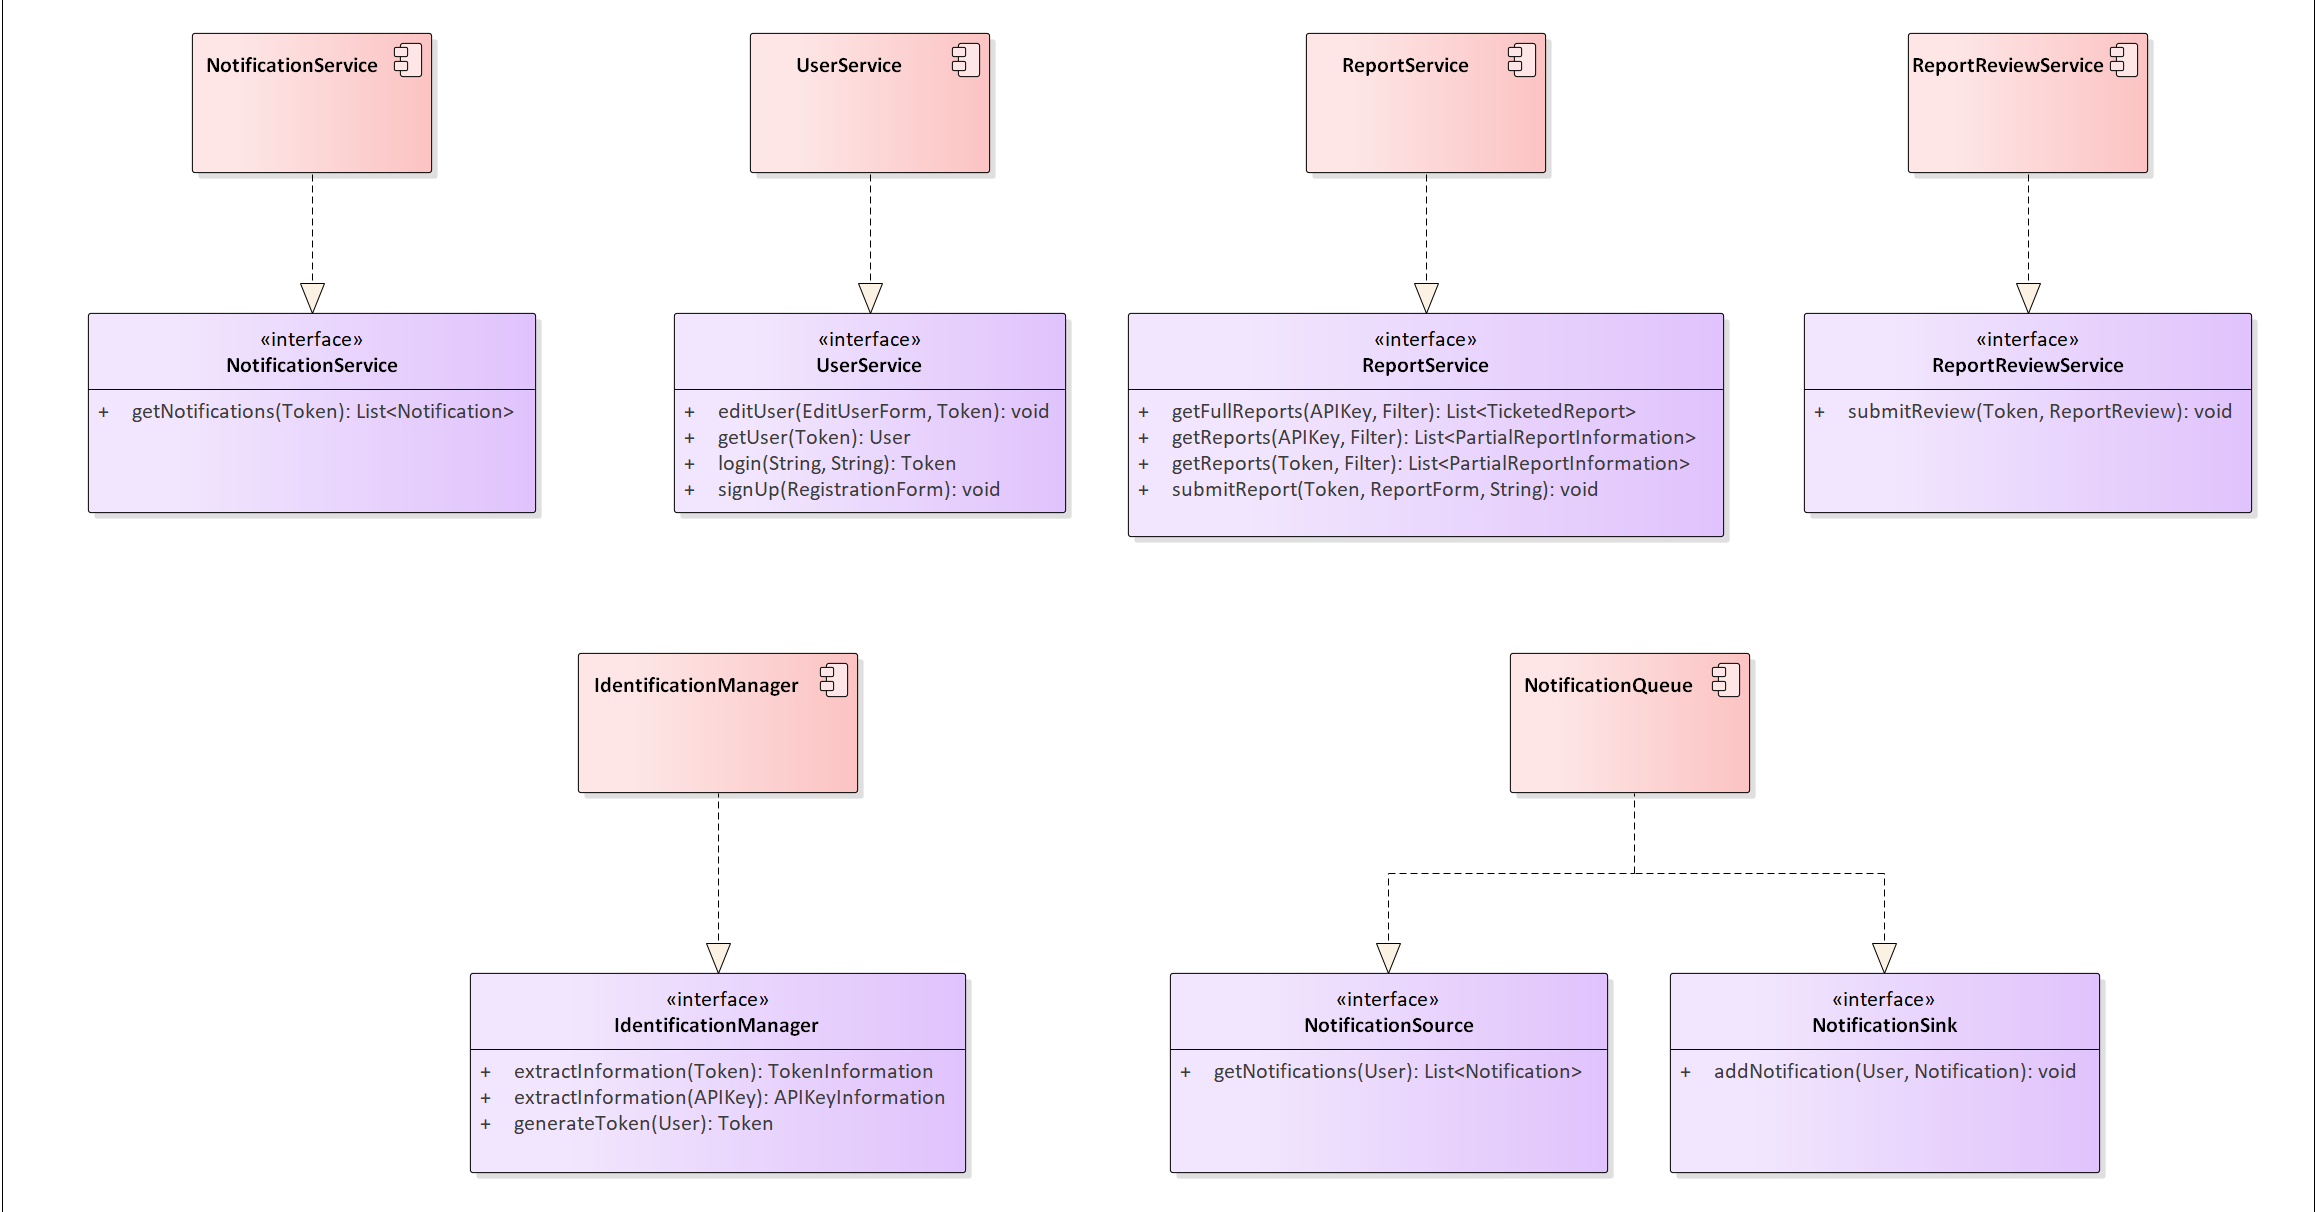
\includegraphics[angle=-90, origin=c, width=0.7\textwidth]{Images/architectural-design/Interfaces 2 of 2.png}}
    \caption{\label{fig:interfaces-2}Component interfaces (2/2).}
\end{figure}

\paragraph{Data model}
The following diagram shows the crucial information contained in the data structures used by the component interfaces. 

\begin{figure}[H]
    \centering
    \fbox{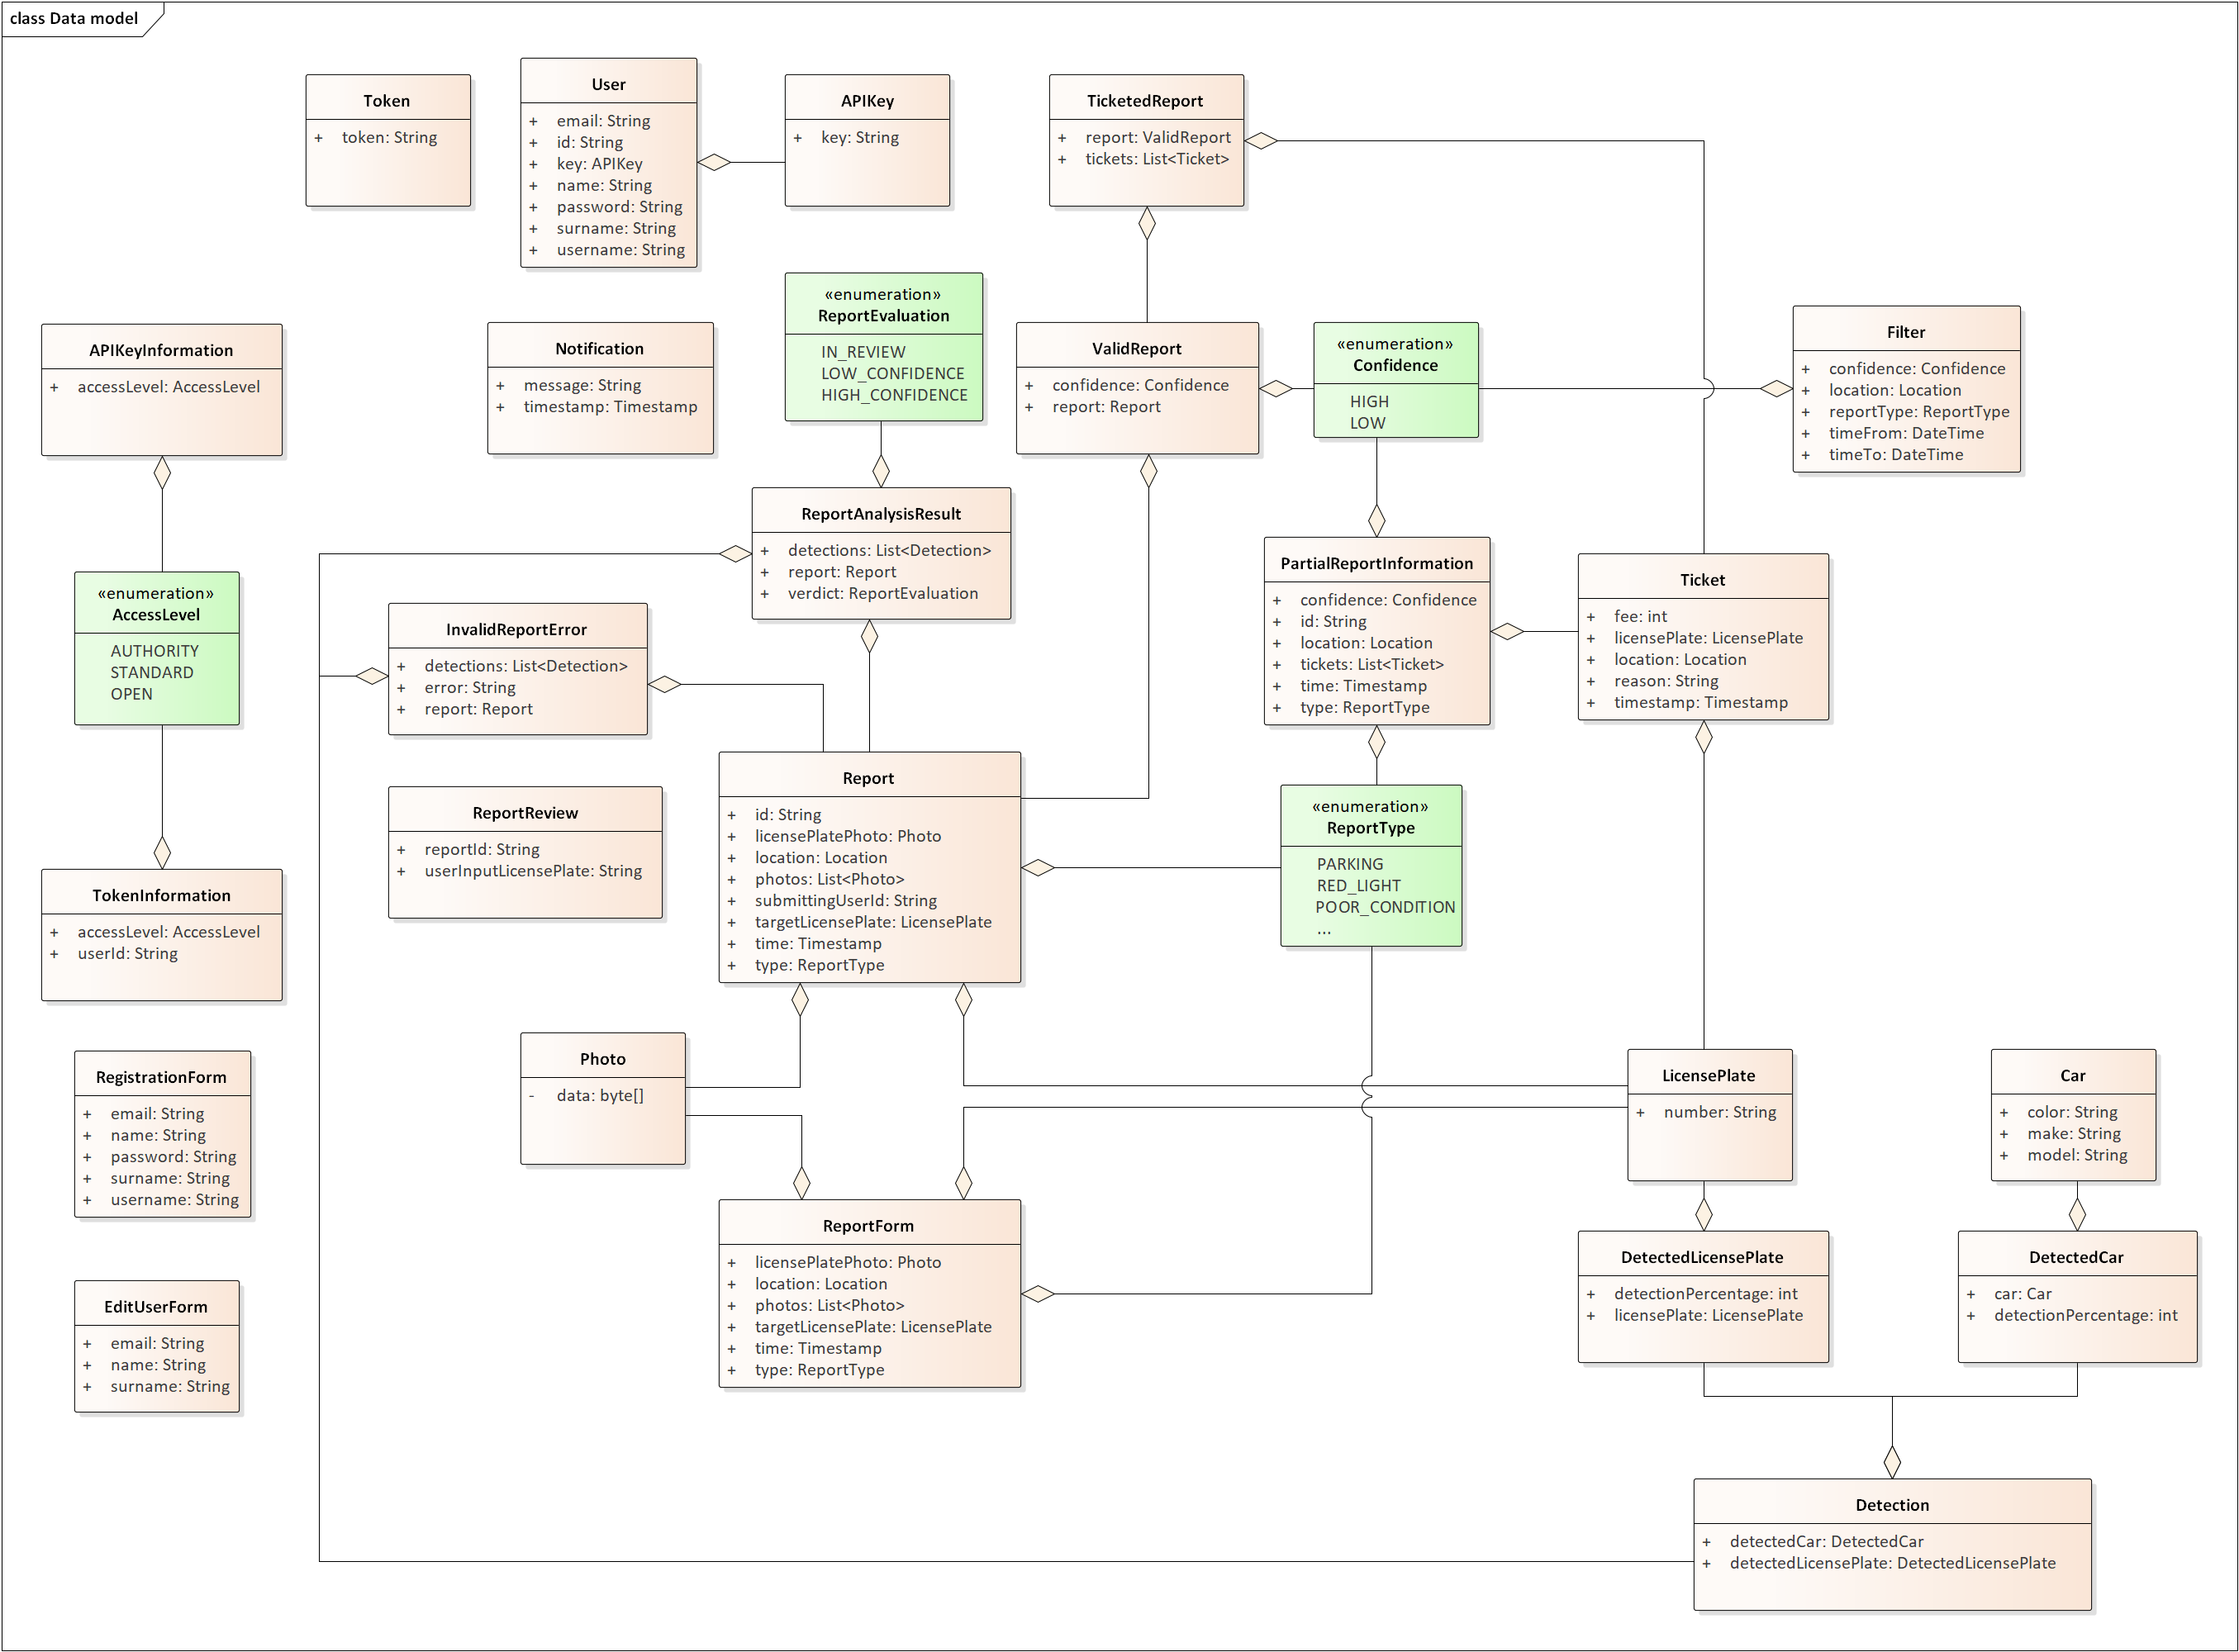
\includegraphics[angle=-90, origin=c, width=0.98\textwidth]{Images/architectural-design/Data model.png}}
    \caption{\label{fig:data-model}Data model diagram.}
\end{figure}

Note that the Token and APIKey are simply strings, how the information provided by them is obtained depends on the implementation. For example, a JSON Web Token would include all relevant data encrypted in the string itself, but the token could also be used as a key to search in the database. How this is done is not relevant, as long as the needed information can be obtained for authentication purposes.

\subsection{Selected architectural styles and patters}

\subsubsection{Architecture patterns}
\begin{itemize}
    \item 
    \textbf{Three tier architecture:} As already mentioned, the SafeStreets system is divided into three tiers: Presentation, Business Logic and Persistence tier.
    \item
    \textbf{Client-Server architecture:} Computing model in which the server hosts, delivers and manages most of the resources and services that are consumed by the clients.

    \begin{figure}[H]
    \centering
    \fbox{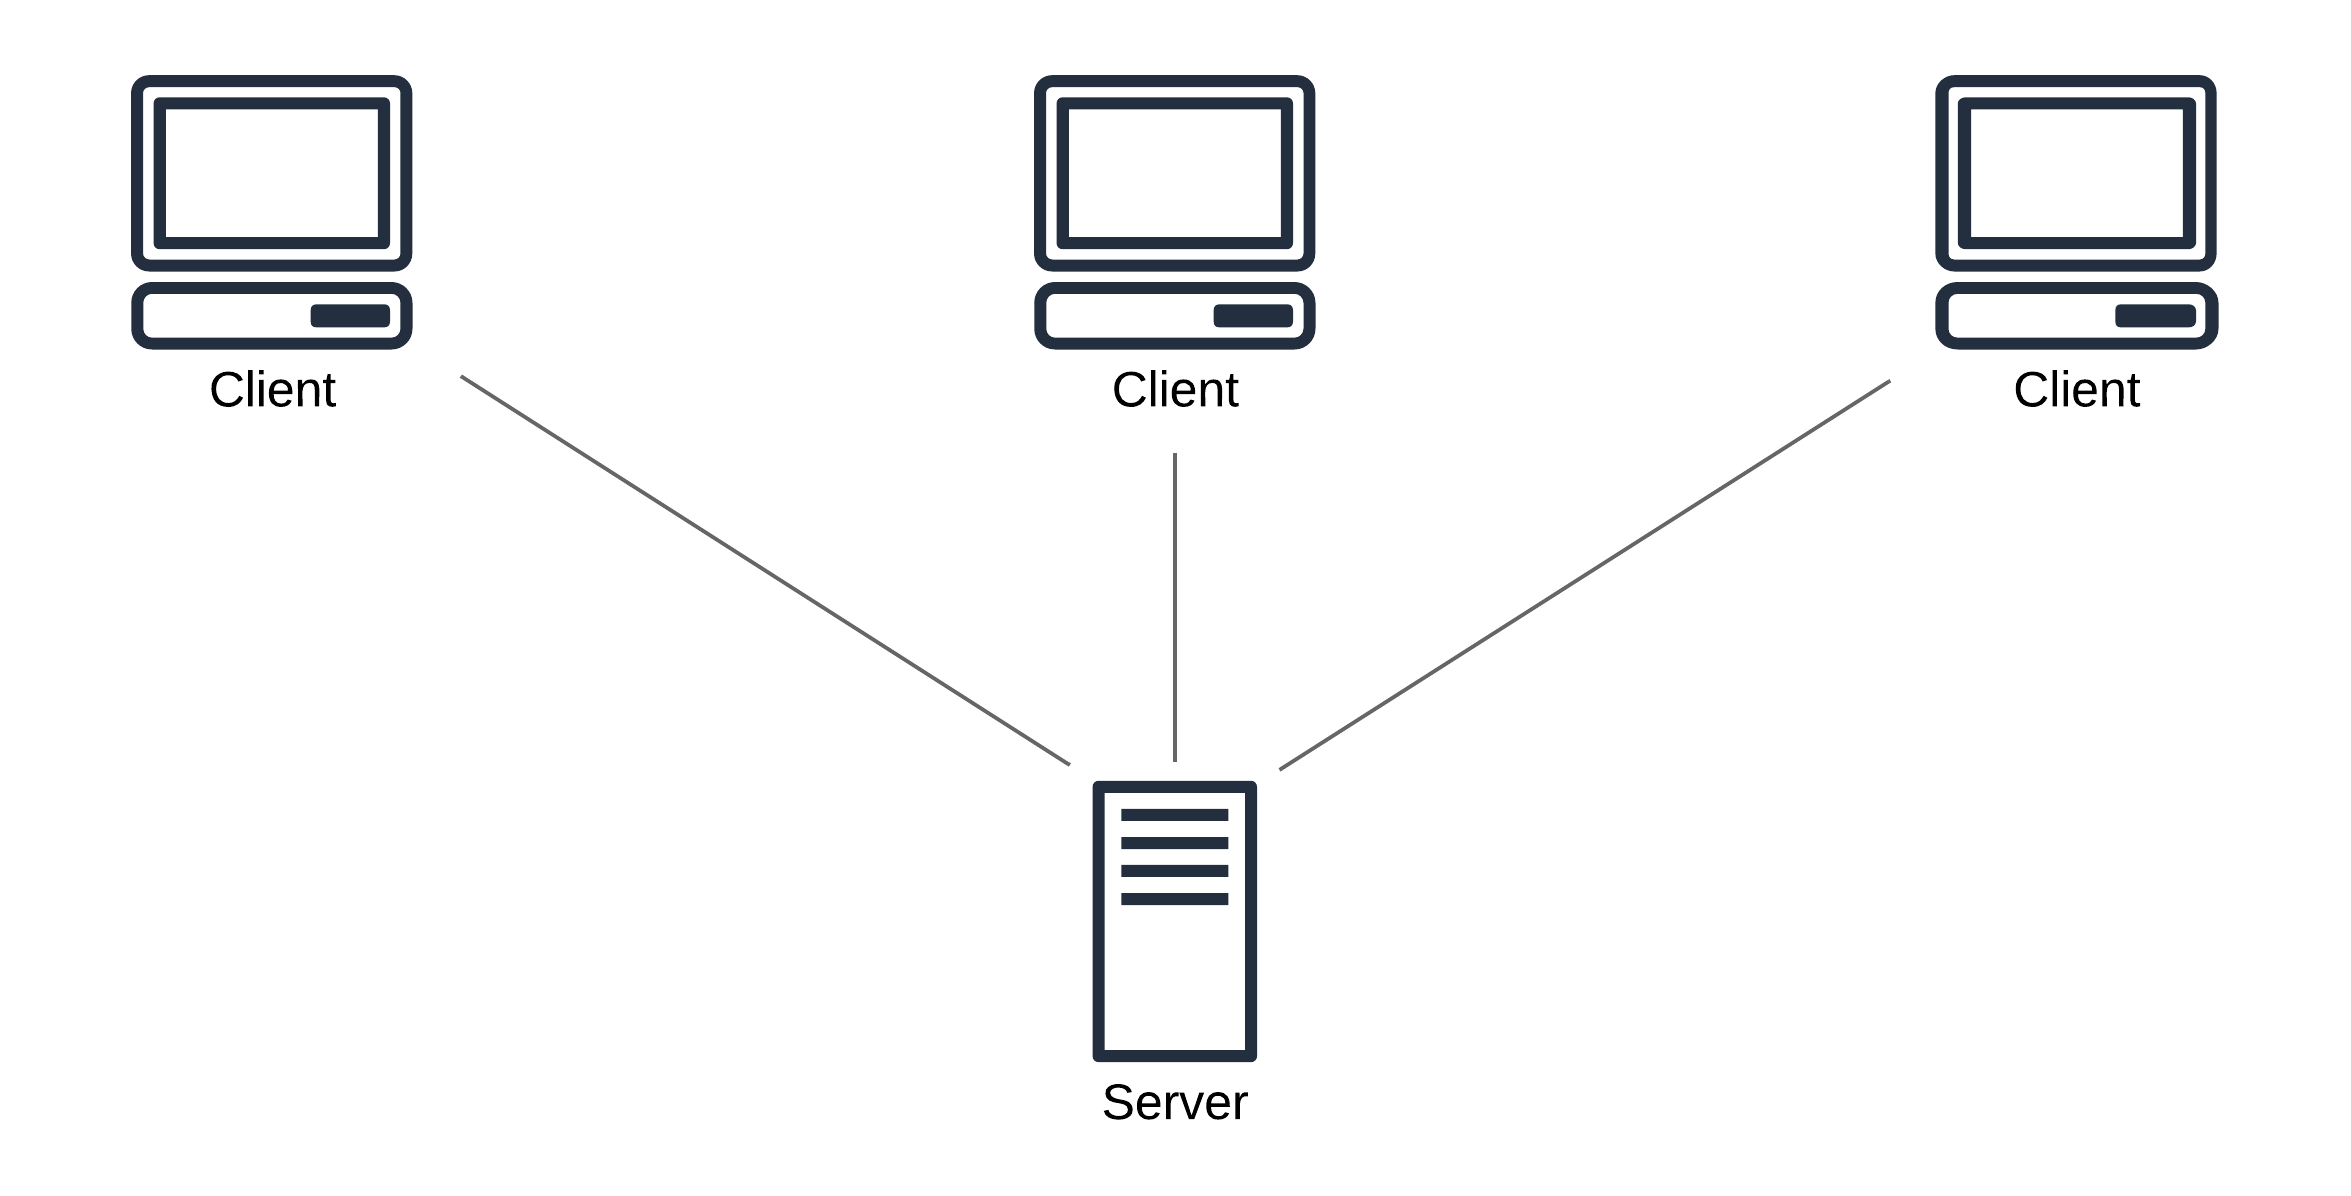
\includegraphics[width=0.8\textwidth]{Images/client-server-architecture.png}}
    \caption{\label{fig:client-server}Client-Server architecture.}
    \end{figure}

    The mobile devices running the application are the clients, which interact with the business logic tier (Application server); it is here that the heavy computation of the system is done. The “Thin Client Server architecture” can also be referenced.
\end{itemize}

\subsubsection{Design patterns}
\begin{itemize}
    \item
    \textbf{Model-View-Controller:} Divides the program logic into three interconnected elements.\\
        \hspace*{3ex}-\hspace*{2ex}Model: Central component. Manages the data, logic and rules of the application.\\
        \hspace*{3ex}-\hspace*{2ex}View: Visual representation of the model.\\
        \hspace*{3ex}-\hspace*{2ex}Controller: Accepts inputs and converts it to commands for the model or view.

    \begin{figure}[H]
    \centering
    \fbox{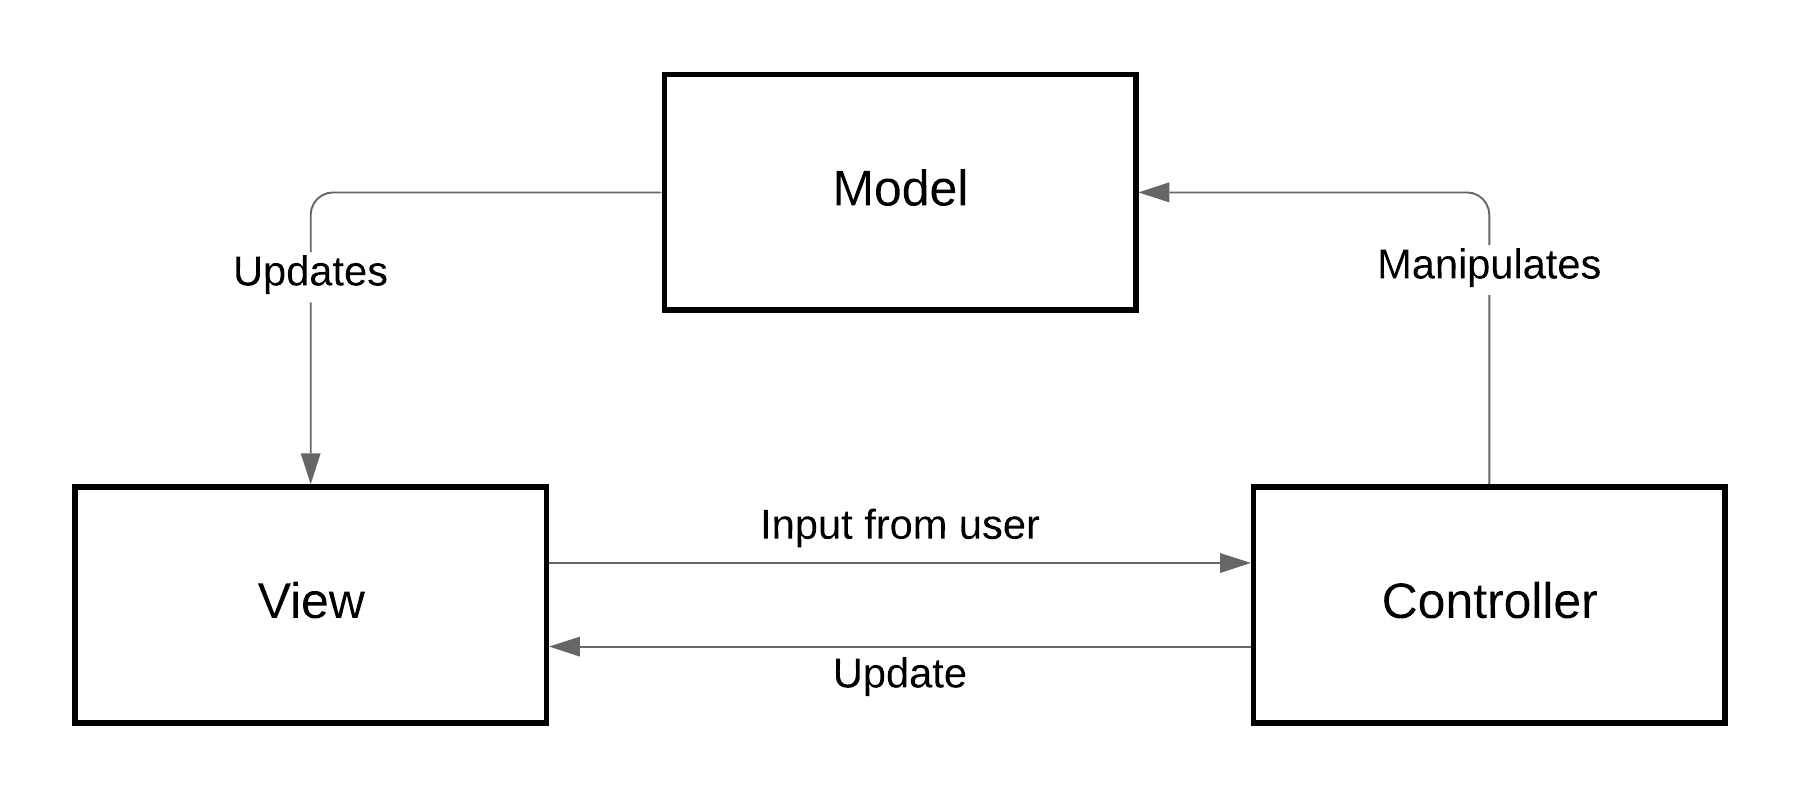
\includegraphics[width=0.8\textwidth]{Images/mvc-pattern.png}}
    \caption{\label{fig:mvc-pattern}Model View Controller pattern.}
    \end{figure}

    This pattern is used in the development of the mobile application, which is the part of the system the user directly interacts with.

    \item
    \textbf{Facade pattern:} Provides a simple interface to a larger body of code. This is used in the backend to expose the API to external users. The router component acts as the facade, interacting with the lower level components and exposing the appropriate endpoints.

    \begin{figure}[H]
    \centering
    \fbox{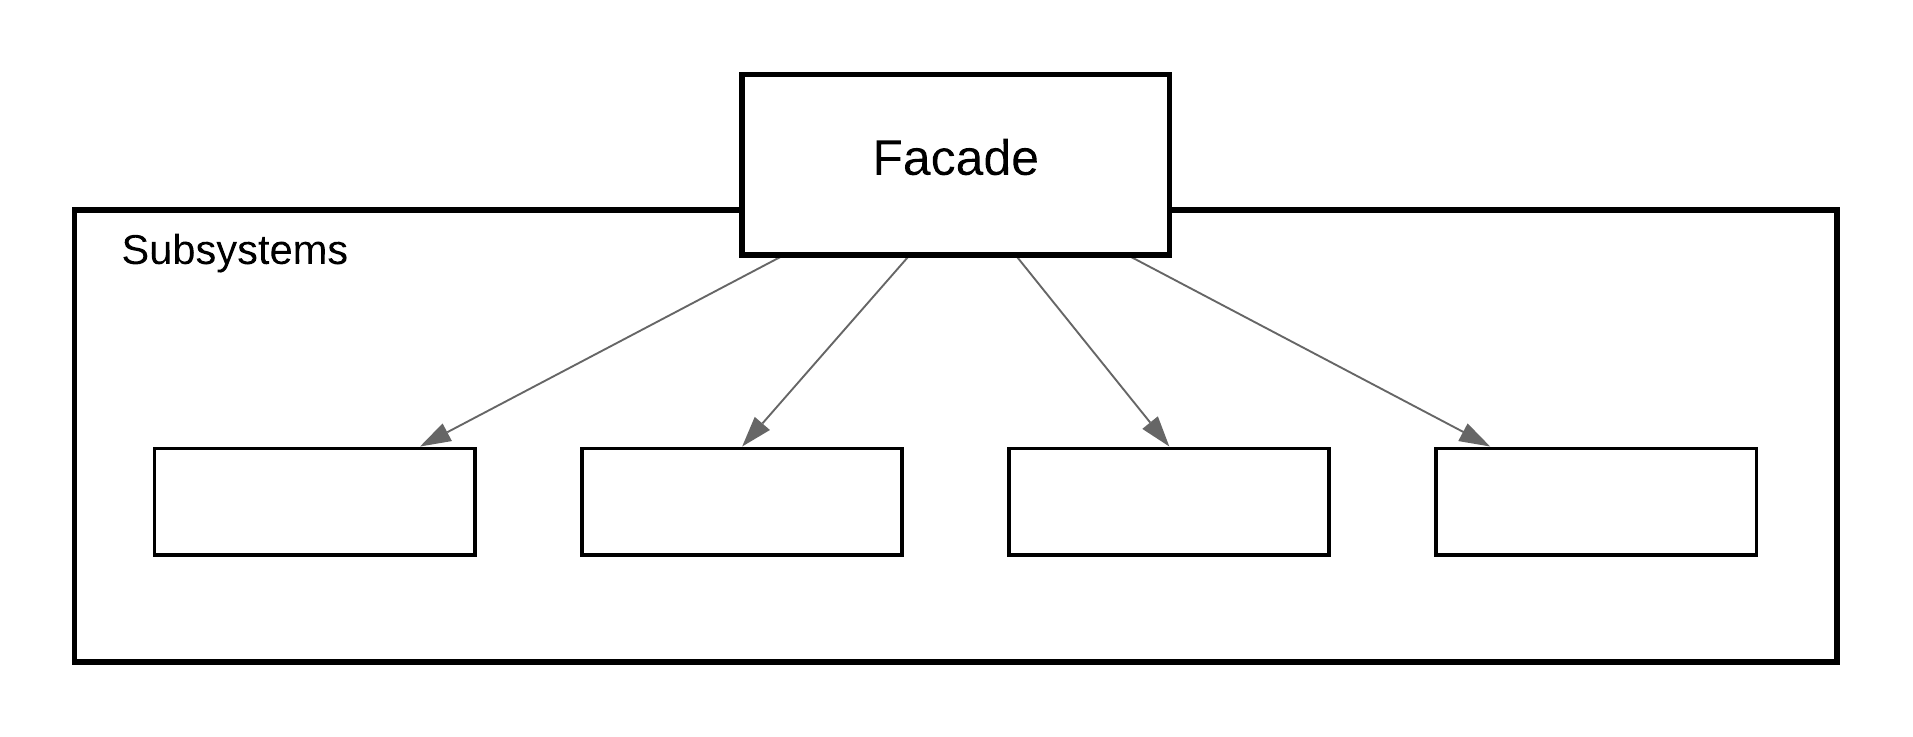
\includegraphics[width=0.8\textwidth]{Images/facade-pattern.png}}
    \caption{\label{fig:facade-pattern}Facade pattern.}
    \end{figure}

    \item
    \textbf{Dependency injection pattern:} A technique whereby one object supplies the dependencies of another object.\\
    Utilized in the backend to solve the dependencies between services.



\end{itemize}